\subsubsection{Análisis de desempeño}
En esta sección analizaremos las destrezas y debilidades del algoritmo en discusión, que posee al menos dos falencias importantes que pueden producir soluciones de deslucida calidad. A continuación las repasamos:

\subsubsubsection{El algoritmo de \textit{sweeping} no prevee el agotamiento de stock}
A medida que un cluster se va construyendo, la capacidad del camión que atenderá los clientes de este conjunto se va agotando, es decir, la sumatoria de las demandas de todos los clientes en el cluster se va aproximando al valor de la capacidad máxima de los camiones. En estos casos, sería ideal emprender la vuelta hacia el depósito con stock suficiente para satisfacer vértices en el camino. Una manera de entender este concepto es visualizar cada ruta como un pétalo, donde la punta del antófilo indica el comienzo del emprendimiento al depósito. De esta manera, se minimiza la distancia recorrida al volver al punto de inicio pero \textbf{satisfaciendo vértices en el proceso}. Desgraciadamente, el algoritmo es inconsciente de esta situación y, en el peor de los casos, puede agotar su stock muy lejos del depósito solamente por seguir a rajatabla la heurística de viajar al nodo angularmente más cercano, pagando una distancia muy alta para volver.

\vskip 8pt

Esta falencia puede ser mitigada con metaheurísticas como \textbf{Tabú Search} o \textbf{Annealing} a la hora de seleccionar el siguiente vértice a visitar, teniendo en cuenta el vecindario inmediato y la cantidad de stock sobrante en el camión.

\begin{figure}[H]
	\centering
	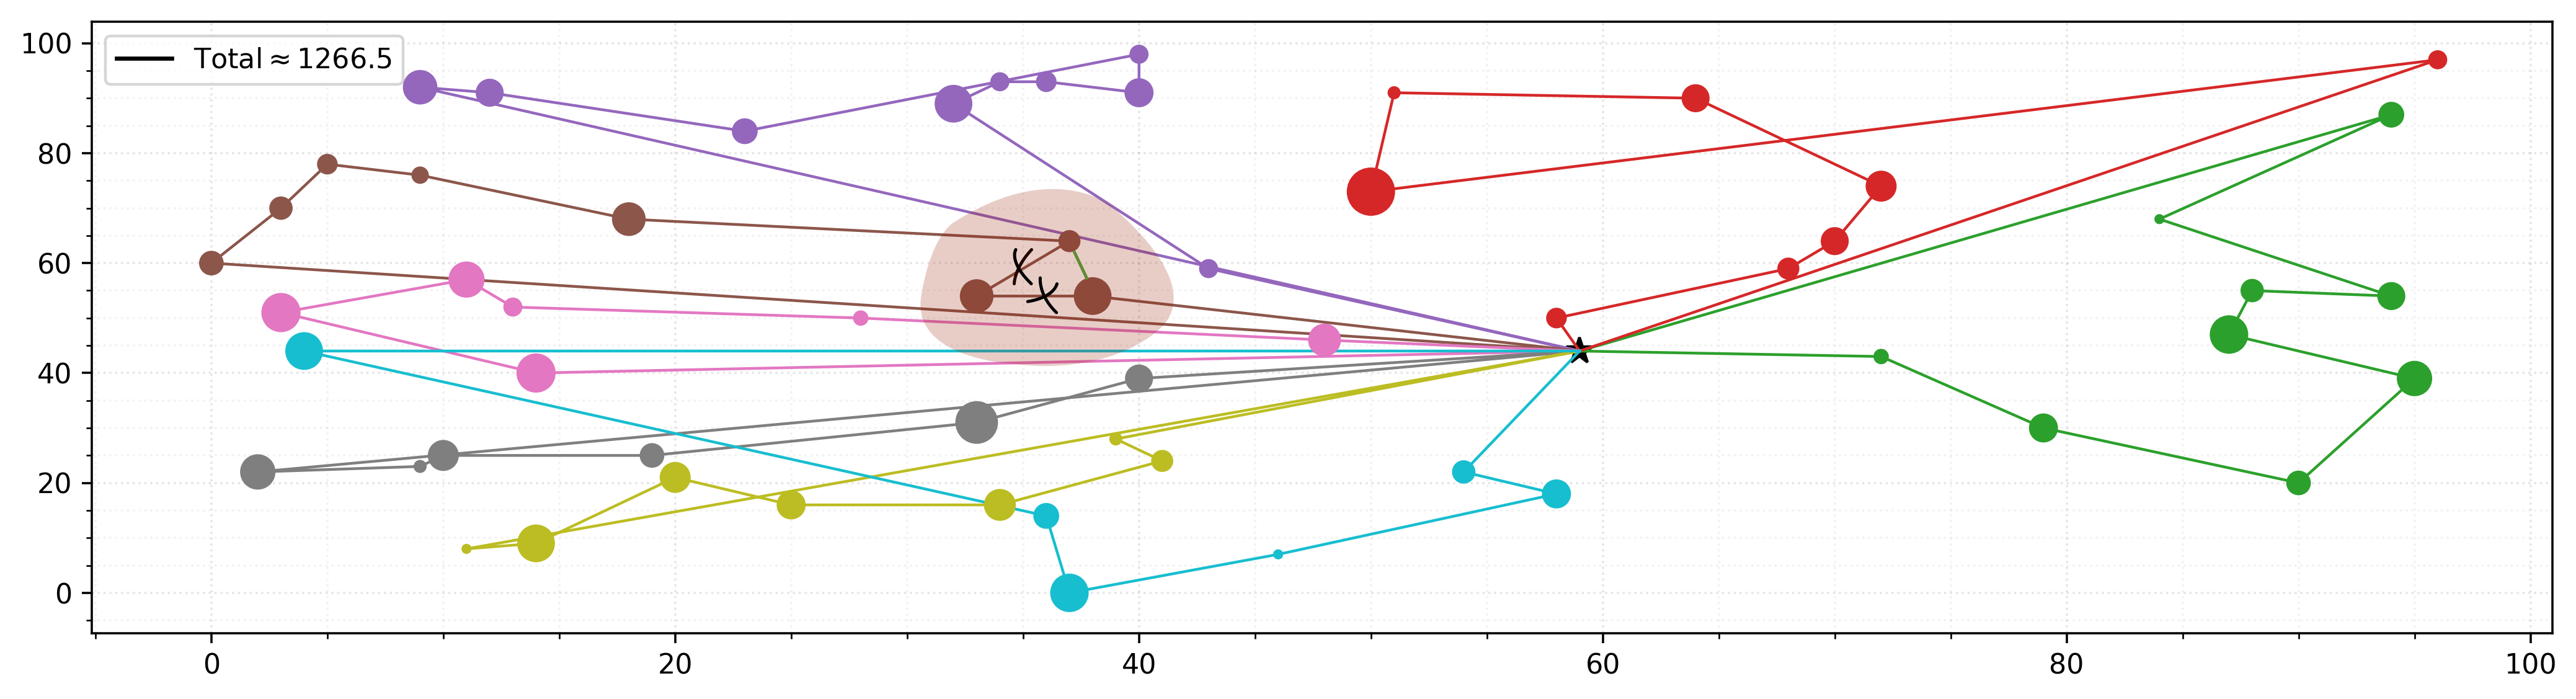
\includegraphics[width=1\textwidth]{sweep/A-n69-k9-emprender-vuelta}
	\caption{\footnotesize Error de optimización en la generación del camino (dataset A-n69-k9)}
	\label{fig:sweep-emprender-vuelta}
\end{figure}

En la figura \ref{fig:sweep-emprender-vuelta} se puede observar que en el camino marrón es posible obtener un mejor recorrido al eliminar los ejes marcados con una cruz y, en cambio, agregando la arista verde como figura en el gráfico. De esta manera quedaría un vértice $v$ sin conectar. Luego, si observamos el eje $e$ formado por el depósito y el nodo más alejado a él en esta ruta, podemos generar una subdivisión de la arista $e$ con el vértice $v$ concluyendo en un camino más óptimo. En resumen: la solución del gráfico \ref{fig:sweep-emprender-vuelta} posee una ruta que realiza un \textit{paso hacia atrás}, alejándose de los nodos que tiene que visitar después y tomando posesión de un cliente que podría haber sido visitado a la hora de \textbf{emprender la vuelta} hacia el depósito. Este ejemplo es uno de los muchos que puede suceder en esta familia de problemas.

\subsubsubsection{La heurística de \textit{TSP} puede ser muy golosa con las distancias}
Debido a que el orden de los clientes en los clusters es resuelto a través de la heurística \textit{Nearest Neighbours} que consiste en visitar el nodo inmediatamente más cercano sobre el cual se está parado, se puede perder el panorama general y cometer decisiones costosas para la calidad de la solución final. El ejemplo más recurrente se ve en la presencia de rutas con bucles o \textit{firuletes}, pues se produce una ``ida y vuelta'' innecesaria con total de visitar el nodo más cercano posible. Esto podría ser evitado utilizado alguna metaheurística como Annealing o Tabú Search para decidir a qué vértice saltar o utilizar una técnica como Lambda Exchange para optimizar e intentar eliminar estas manifestaciones del problema descripto. Analizaremos este fenómeno gráficamente:

\begin{figure}[H]
	\centering
	\begin{minipage}{0.48\textwidth}
		\centering
		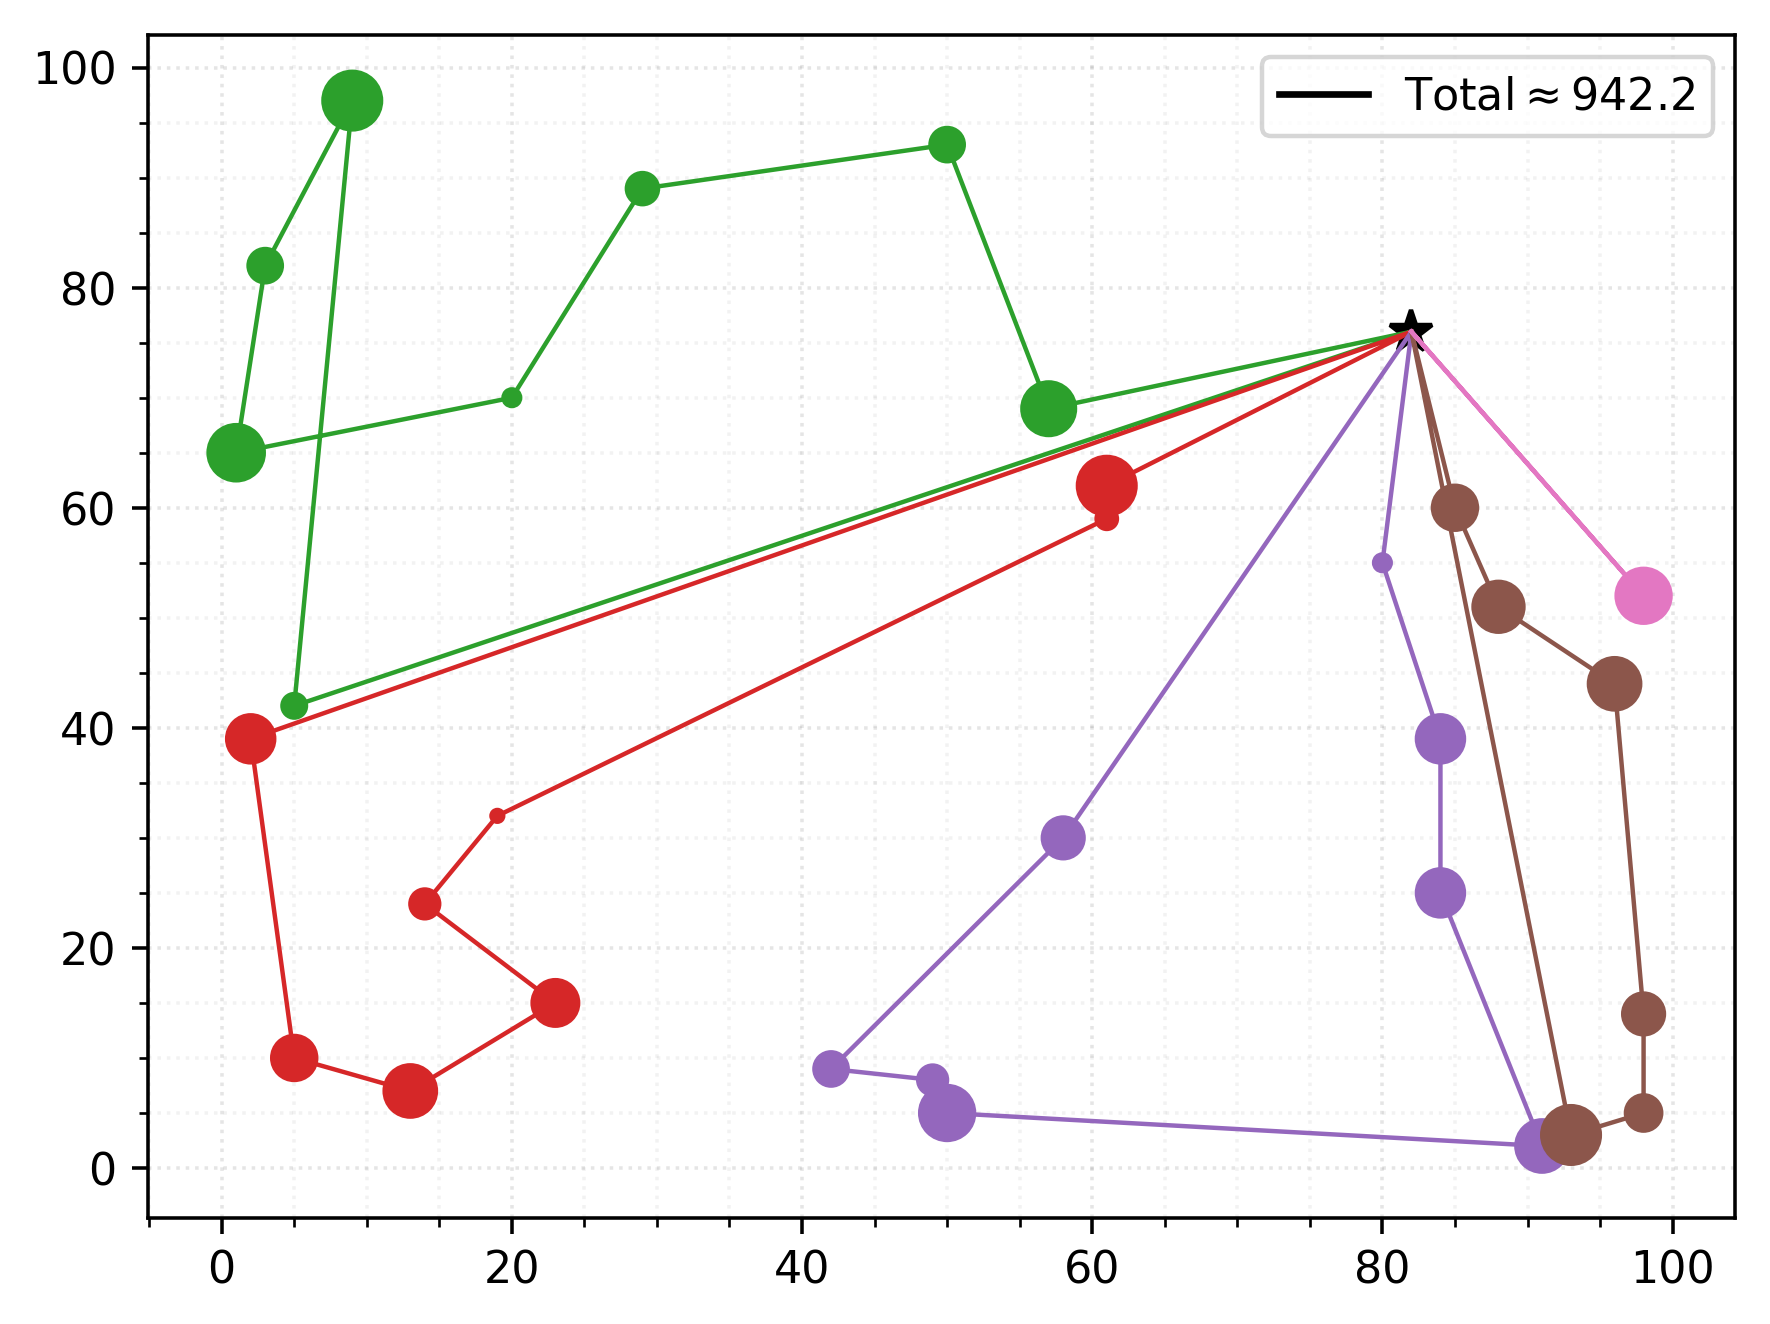
\includegraphics[width=1\textwidth]{sweep/sweep-A-n32-k5}
	\end{minipage}%
	\hspace{0.03\textwidth}
	\begin{minipage}{0.48\textwidth}
    \caption{\footnotesize Sweeping no adaptativo}
		\label{fig:sweep-without-adaptative}
		En este ejemplo se puede ver claramente la aparición de un circuito en la ruta verde. Como ya fue explicado, este se debe a que el algoritmo de resolución del TSP busca los nodos inmediatamente más cercanos sin considerar otras alternativas (a priori más ineficientes) pero que a la larga resultan más óptimas. Al seguir a rajatabla la heurística de \textit{Nearest Neighbours}, se comete un error de \textit{tunnel view} y se ignoran alternativas más eficientes a la larga.
	\end{minipage}%
\end{figure}

\subsubsubsection{Clusterización con sweeping adaptativo vs sin sweeping adaptativo}
En la figura \ref{fig:sweep-with-adaptative} se puede observar una clusterización correcta de los vértices. Los nodos recorridos por el camión verde son cercanos entre sí y lo mismo sucede con los del camión rojo. En cambio, en la figura \ref{fig:sweep-without-adaptative}, se puede observar cómo los clusters se interponen entre sí debido a que se comenzó a barrer angularmente sobre ángulo $0$, interrumpiendo a la mitad la concepción de un cluster óptimo.
\begin{figure}[H]
	\centering
	\begin{minipage}{0.48\textwidth}
		\centering
		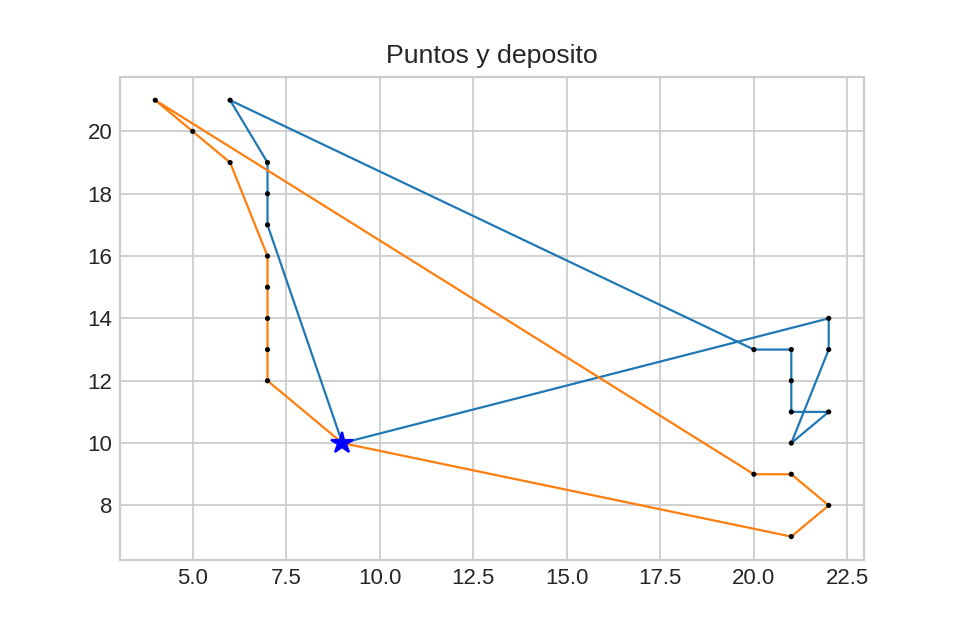
\includegraphics[width=1\textwidth]{sweep/sweep-without-adaptative}
		\caption{\footnotesize Sweeping no adaptativo}
		\label{fig:sweep-without-adaptative}
	\end{minipage}%
	\hspace{0.03\textwidth}
	\begin{minipage}{0.48\textwidth}
		\centering
		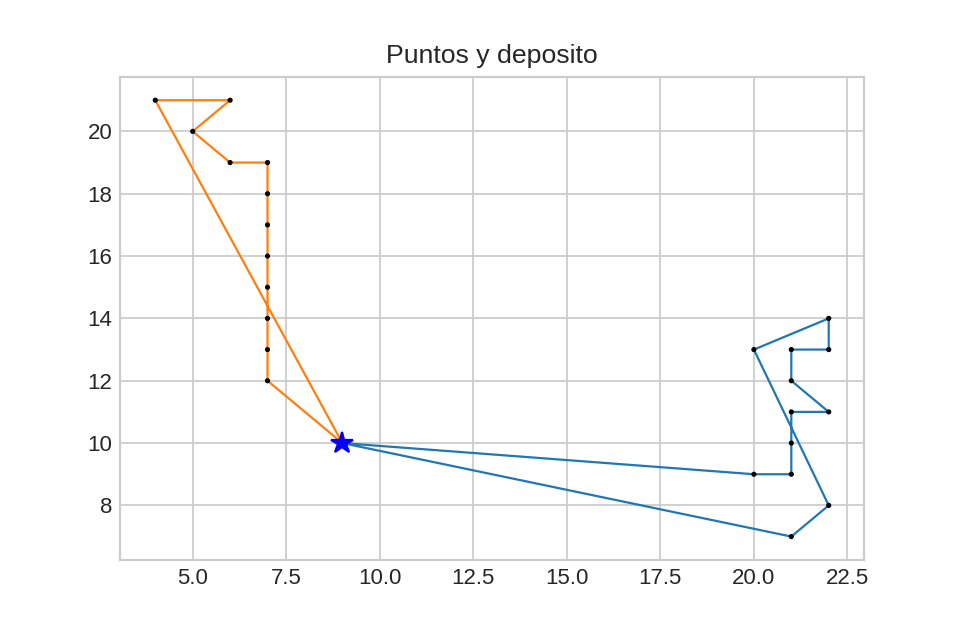
\includegraphics[width=1\textwidth]{sweep/sweep-with-adaptative}
		\caption{\footnotesize Sweeping adaptativo}
		\label{fig:sweep-with-adaptative}
	\end{minipage}%
\end{figure}

\subsubsubsection{El barrido angular puede clusterizar vértices muy lejanos entre sí}
Dada la clusterizaciónn de vértices $V=\{v_{1}, \dots, v_{n}\}$ realizada por la heurística de Sweeping donde, si bien está asegurado que la distancia angular desde el depósito entre todo $v_{i}$ y $v_{i+1}$ con $1 \leq i < n$ es mínima en todo el grafo, no está asegurado que la distancia euclidiana entre $v_{i}$ y $v_{i+1}$ sea mínima también. De hecho, la distancia entre $v_{i}$ y $v_{i+1}$ puede ser arbitraria. Sin embargo, al clusterizar ambos vértices juntos, estamos firmando un contrato donde un solo camión deberá proveer a ambos y esto puede ser extremadamente costoso por más que los recorridos sean realizados a fin de cuentas con una heurística de TSP. Veamos un ejemplo:

\begin{figure}[H]
	\centering
	\begin{minipage}{0.48\textwidth}
		\centering
		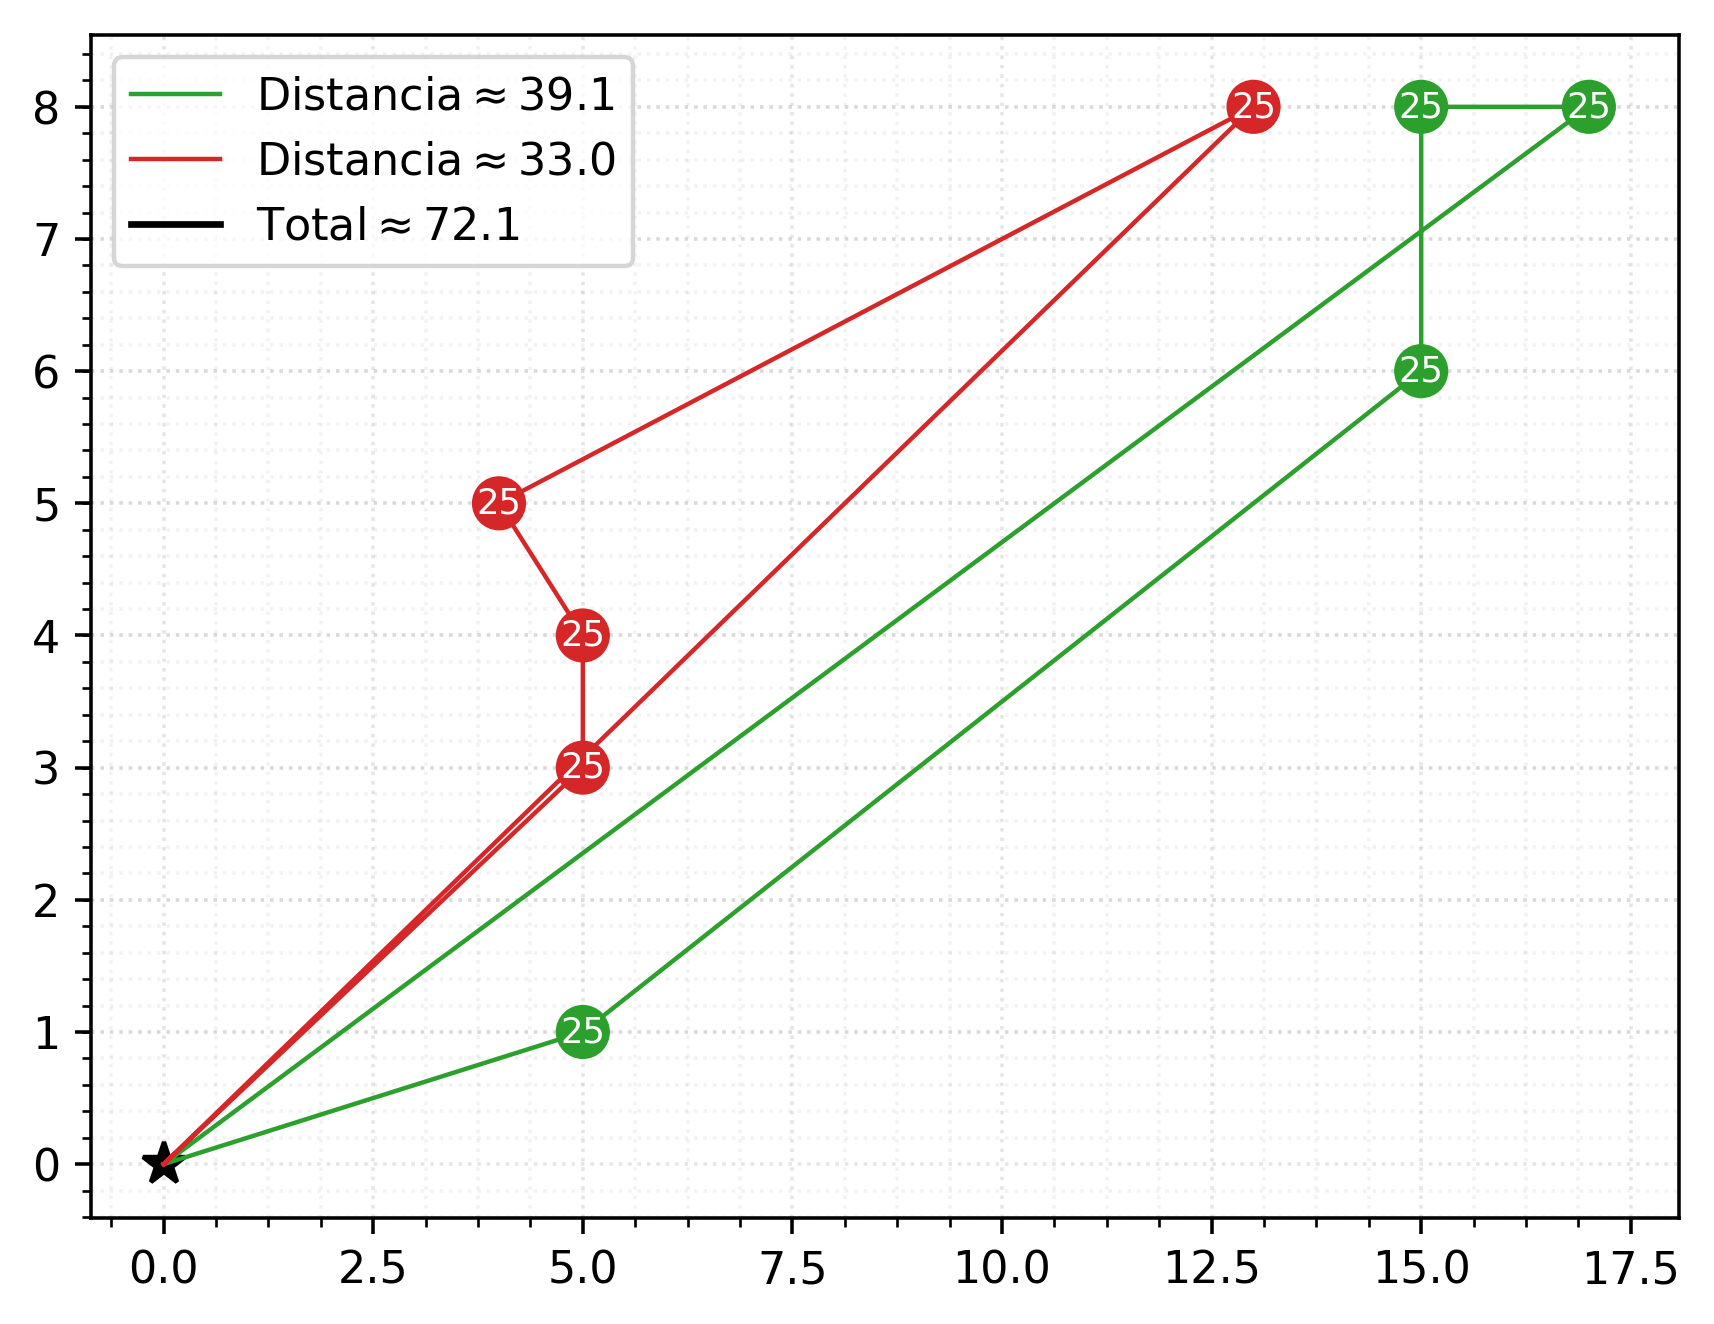
\includegraphics[width=1\textwidth]{sweep/sw-custom-n9-sweep-close-angular-far-euclidean}
		\caption{\footnotesize Sweeping + Nearest Neighbours. Capacidad 100.}
		\label{fig:sw-custom-n9-sweep-close-angular-far-euclidean}
	\end{minipage}%
	\hspace{0.03\textwidth}
	\begin{minipage}{0.48\textwidth}
		\centering
		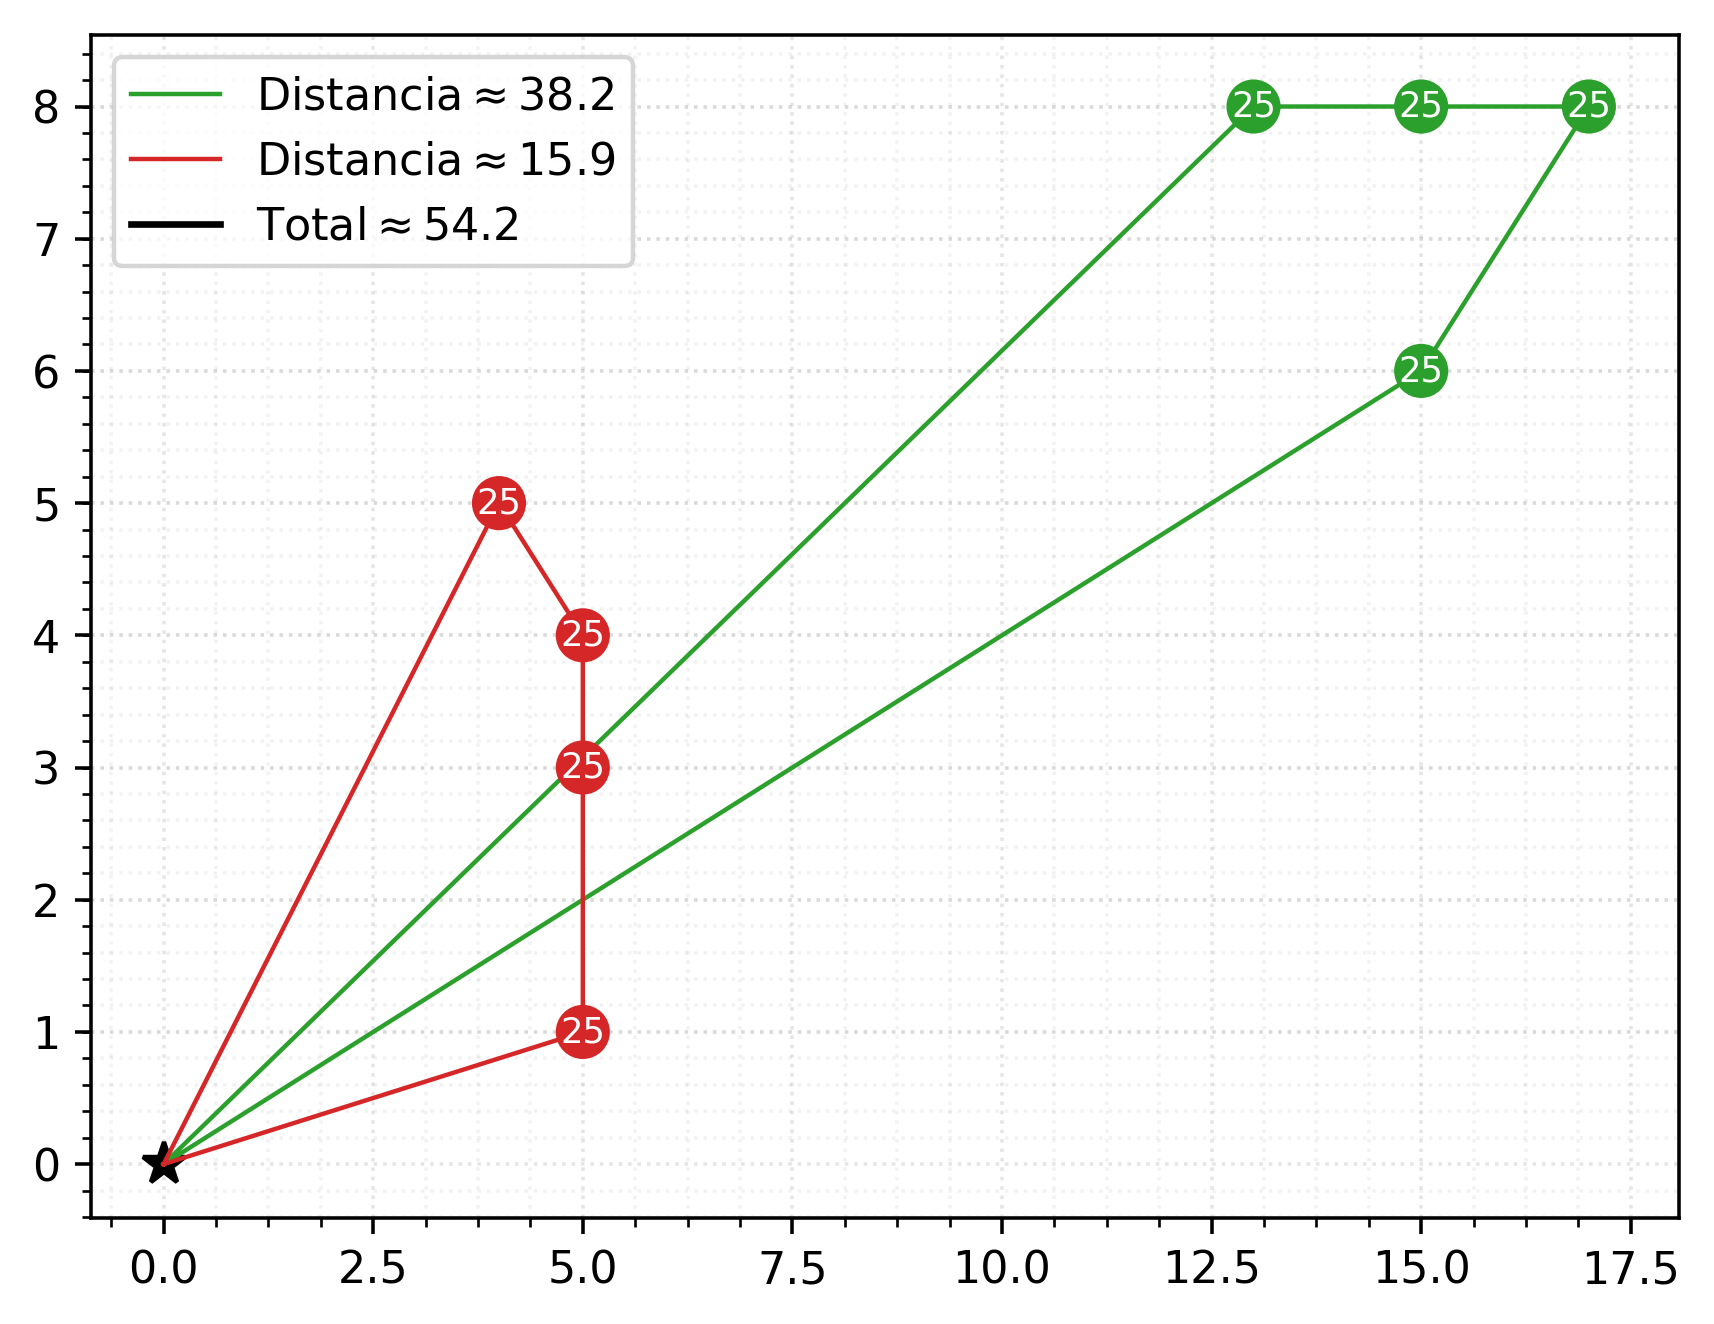
\includegraphics[width=1\textwidth]{sweep/km-custom-n9-sweep-close-angular-far-euclidean}
		\caption{\footnotesize K-Means + Nearest Neighbours. Capacidad 100.}
		\label{fig:km-custom-n9-sweep-close-angular-far-euclidean}
	\end{minipage}%
\end{figure}

En este caso se puede observar claramente lo mencionado. La solución con \textit{sweeping} encuentra primero el vértice $(5, 1)$ e inmediatamente después el $(15, 6)$, seguido del $(17, 8)$ y cierra el cluster con $(15, 8)$. Luego ya se disponen de 4 vértices cuya demanda suma $100$, la capacidad máxima de un camión. Esto forma un cluster de cuatro vértices donde uno de ellos está muy lejos de los otros tres pues estos cuatro son consecutivos angularmente pero \textbf{no} euclideanamente. Lo mismo sucede con los otros cuatro vértices sobrantes del grafo. En consecuencia, se consume mucha distancia yendo y viniendo de aquellos vértices lejanos del resto. En cambio, en la figura \ref{fig:km-custom-n9-sweep-close-angular-far-euclidean} se puede observar una distribución más natural de las rutas y, en consecuencia, un decremento en la distancia total recorrida por ellas. Esto se debe a que se utilizó la heurística de clusterización \textbf{K-Means} que resulta \textbf{más apropiada para la instancia del problema} pues – como será explicado más adelante – construye los clusters a partir de la distancia euclideana entre sus vértices y no sus distancias angulares al depósito.

\subsubsubsection{Análisis de instancias generales}
A continuación pondremos a prueba esta heurística con algunas instancias de los datasets \textbf{A} y \textbf{B} provistos por la cátedra. A la izquierda, la solución del algoritmo \textbf{Clusterize First (Sweep), Route Second (Nearest Neighbours)}. A la derecha, la solución óptima conocida.

\begin{figure}[H]
	\begin{minipage}{0.15\textwidth}
		\centering
		\textbf{Instancia}
	\end{minipage}%
	\begin{minipage}{0.40\textwidth}
		\centering
		\textbf{Soluciones golosas}
	\end{minipage}%
	\hspace{0.03\textwidth}
	\begin{minipage}{0.40\textwidth}
		\centering
		\textbf{Soluciones golosas}
	\end{minipage}%
\end{figure}

\begin{figure}[H]
	\begin{minipage}{0.15\textwidth}
		\centering
		\texttt{A-n32-k5}
	\end{minipage}%
	\begin{minipage}{0.40\textwidth}
		\centering
		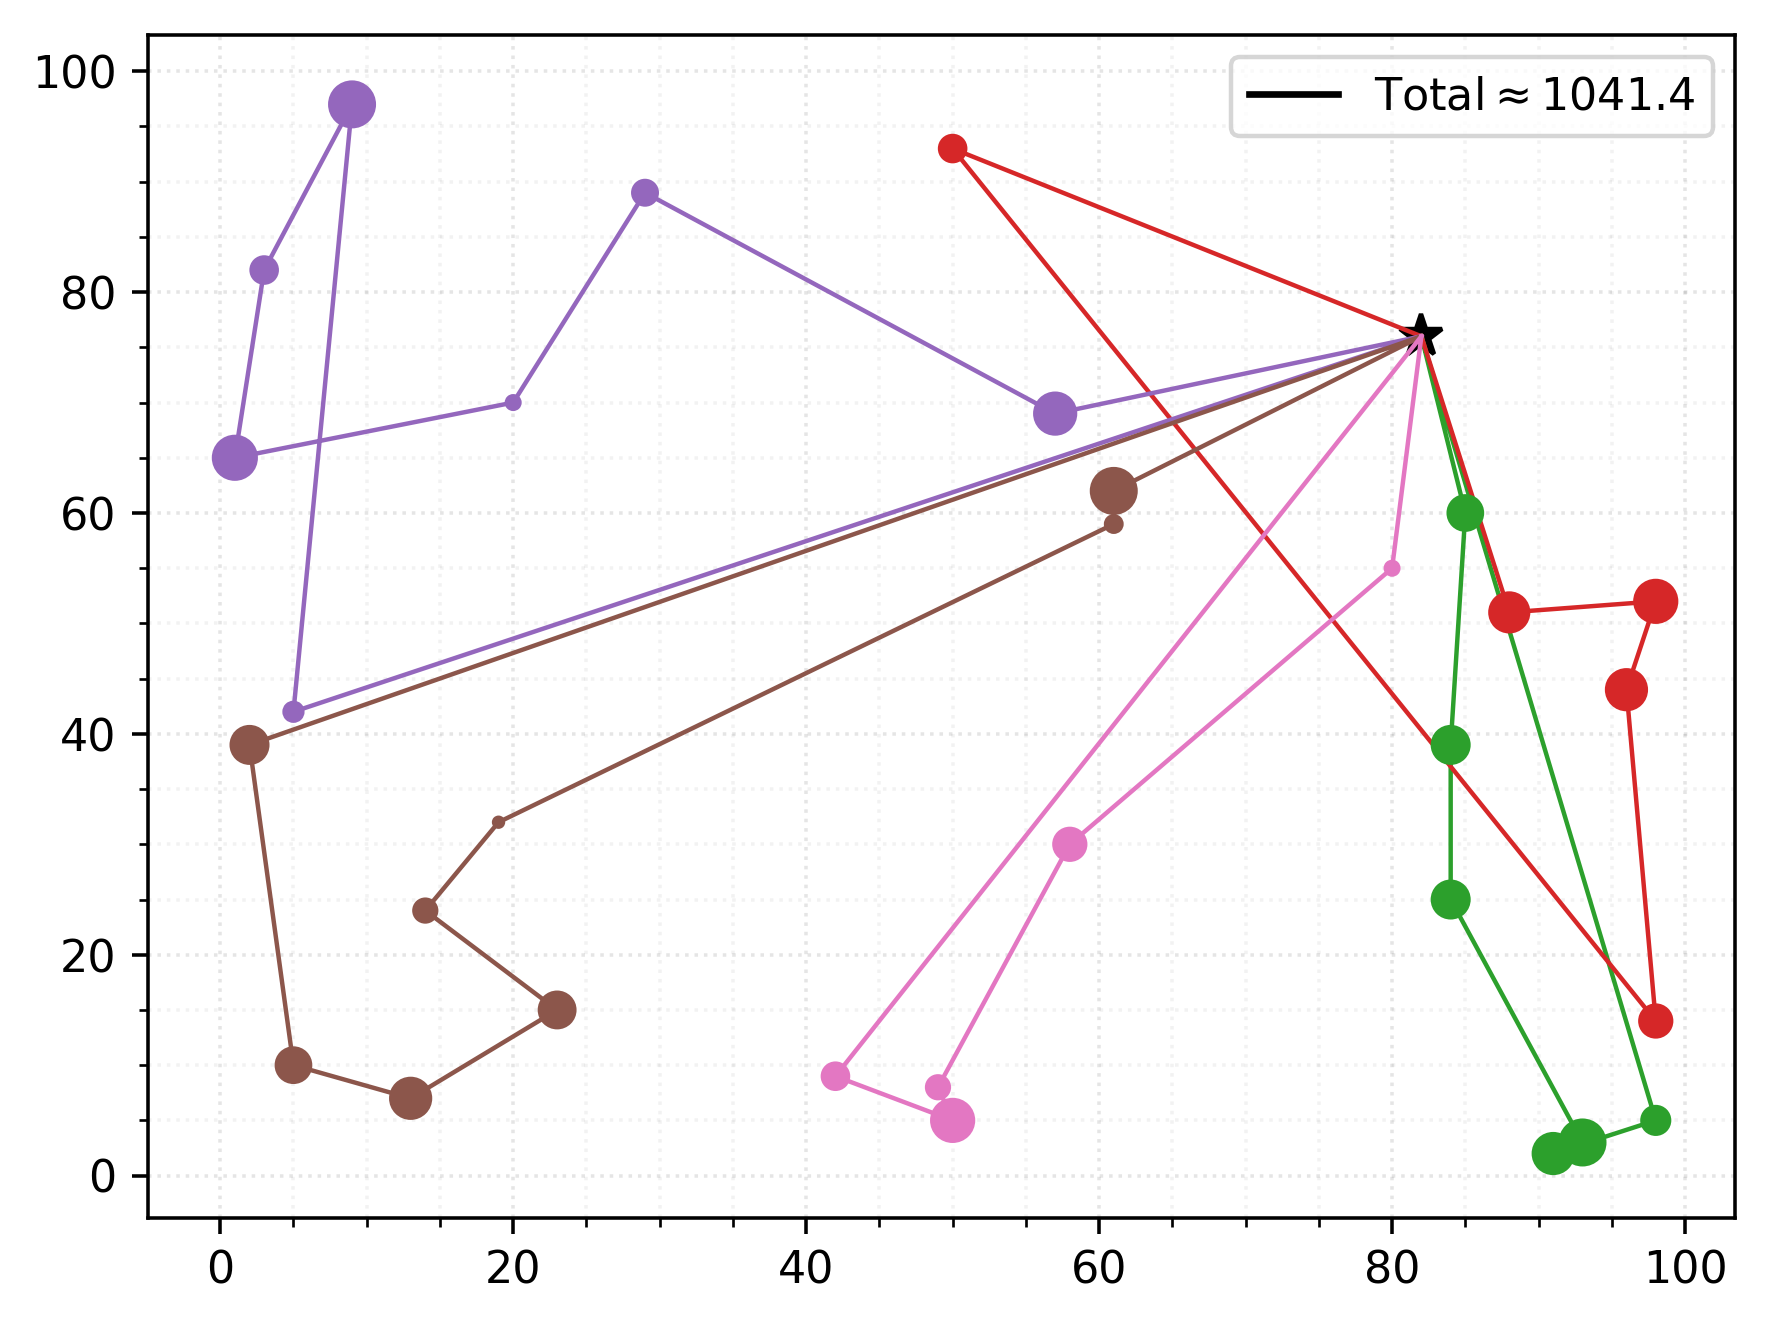
\includegraphics[width=\linewidth]{sweep/sw-A-n32-k5}\par
	\end{minipage}%
	\hspace{0.03\textwidth}
	\begin{minipage}{0.40\textwidth}
		\centering
		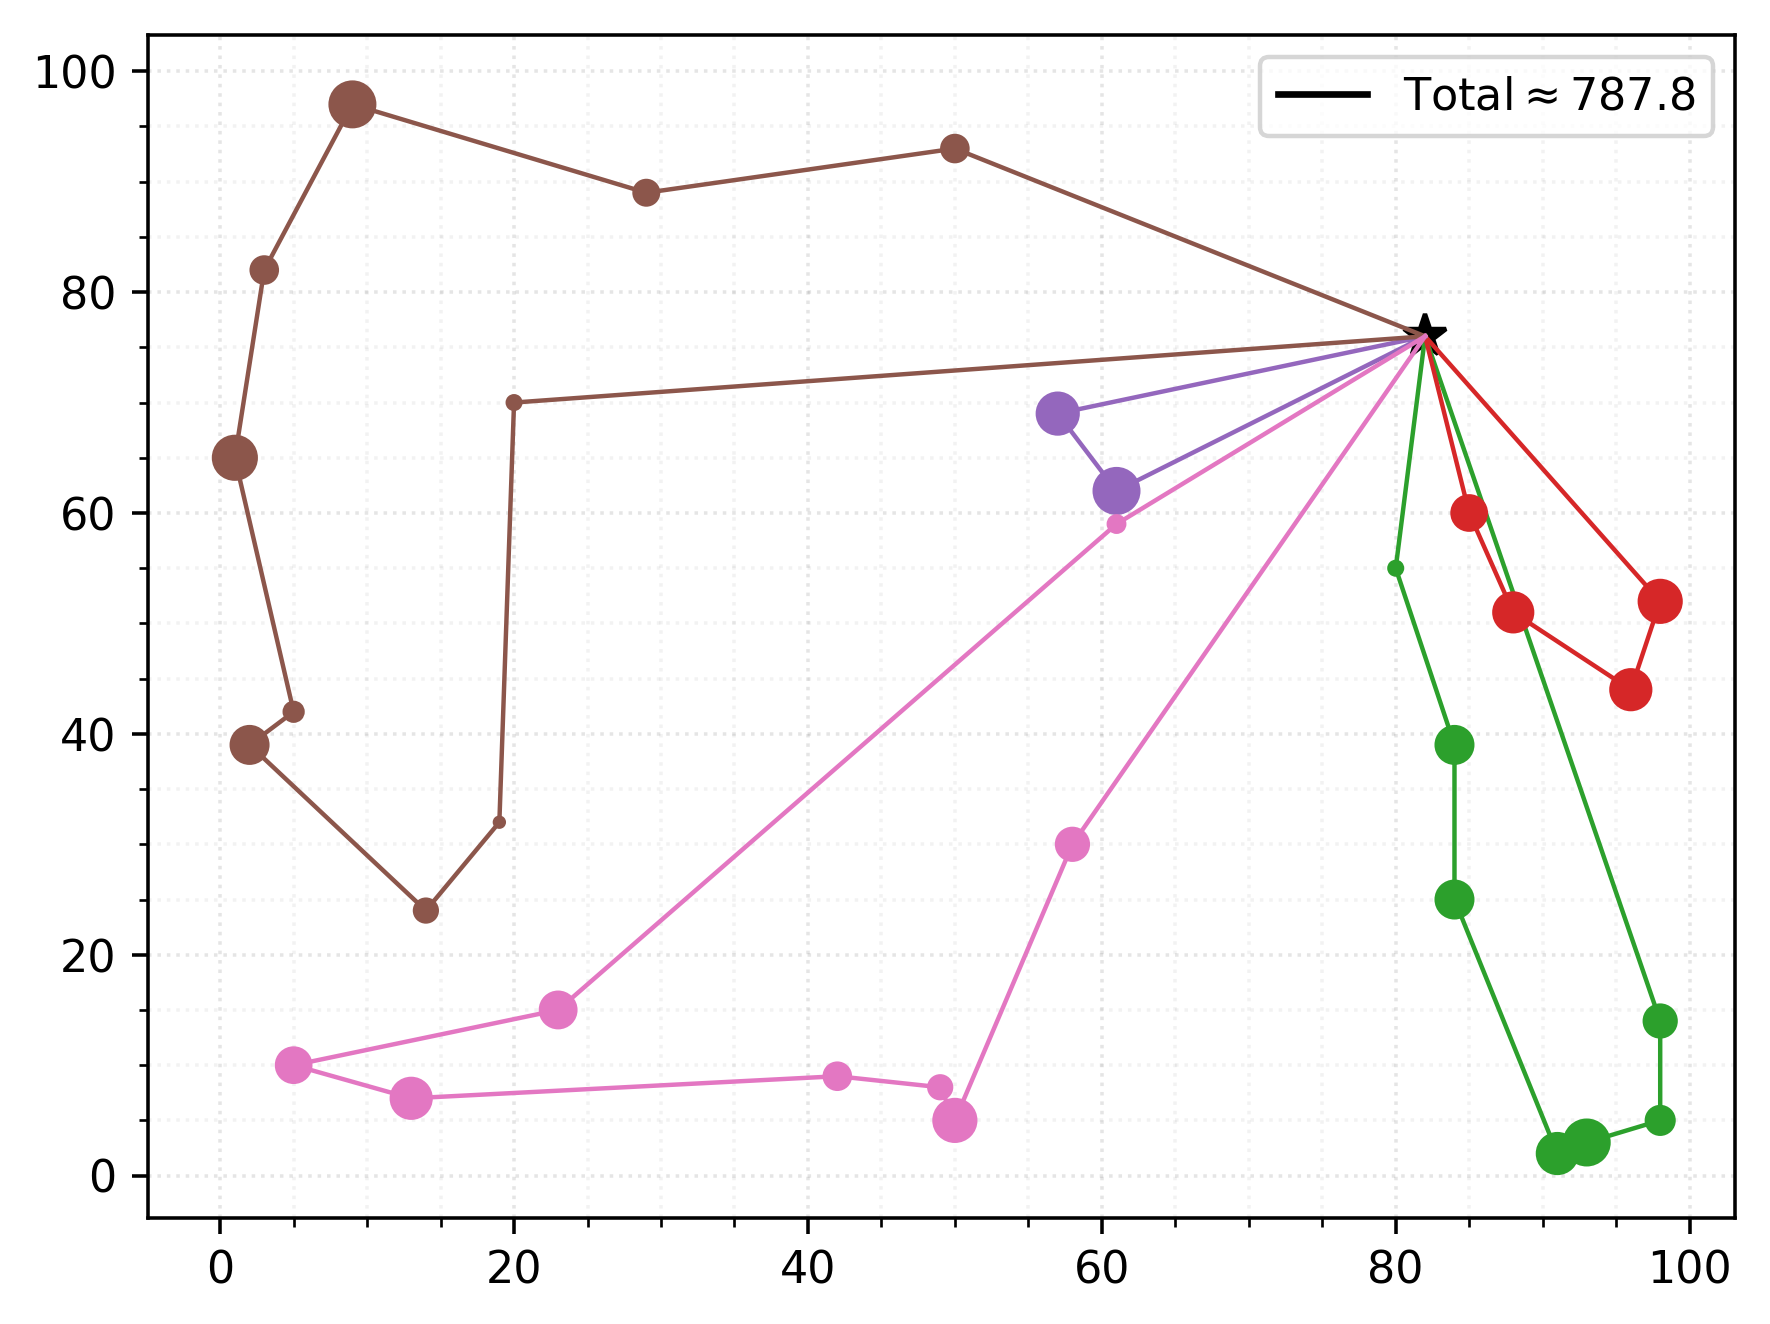
\includegraphics[width=\linewidth]{A-n32-k5-optima}\par
	\end{minipage}%
\end{figure}

\begin{figure}[H]
	\begin{minipage}{0.15\textwidth}
		\centering
		\texttt{A-n38-k5}
	\end{minipage}%
	\begin{minipage}{0.40\textwidth}
		\centering
		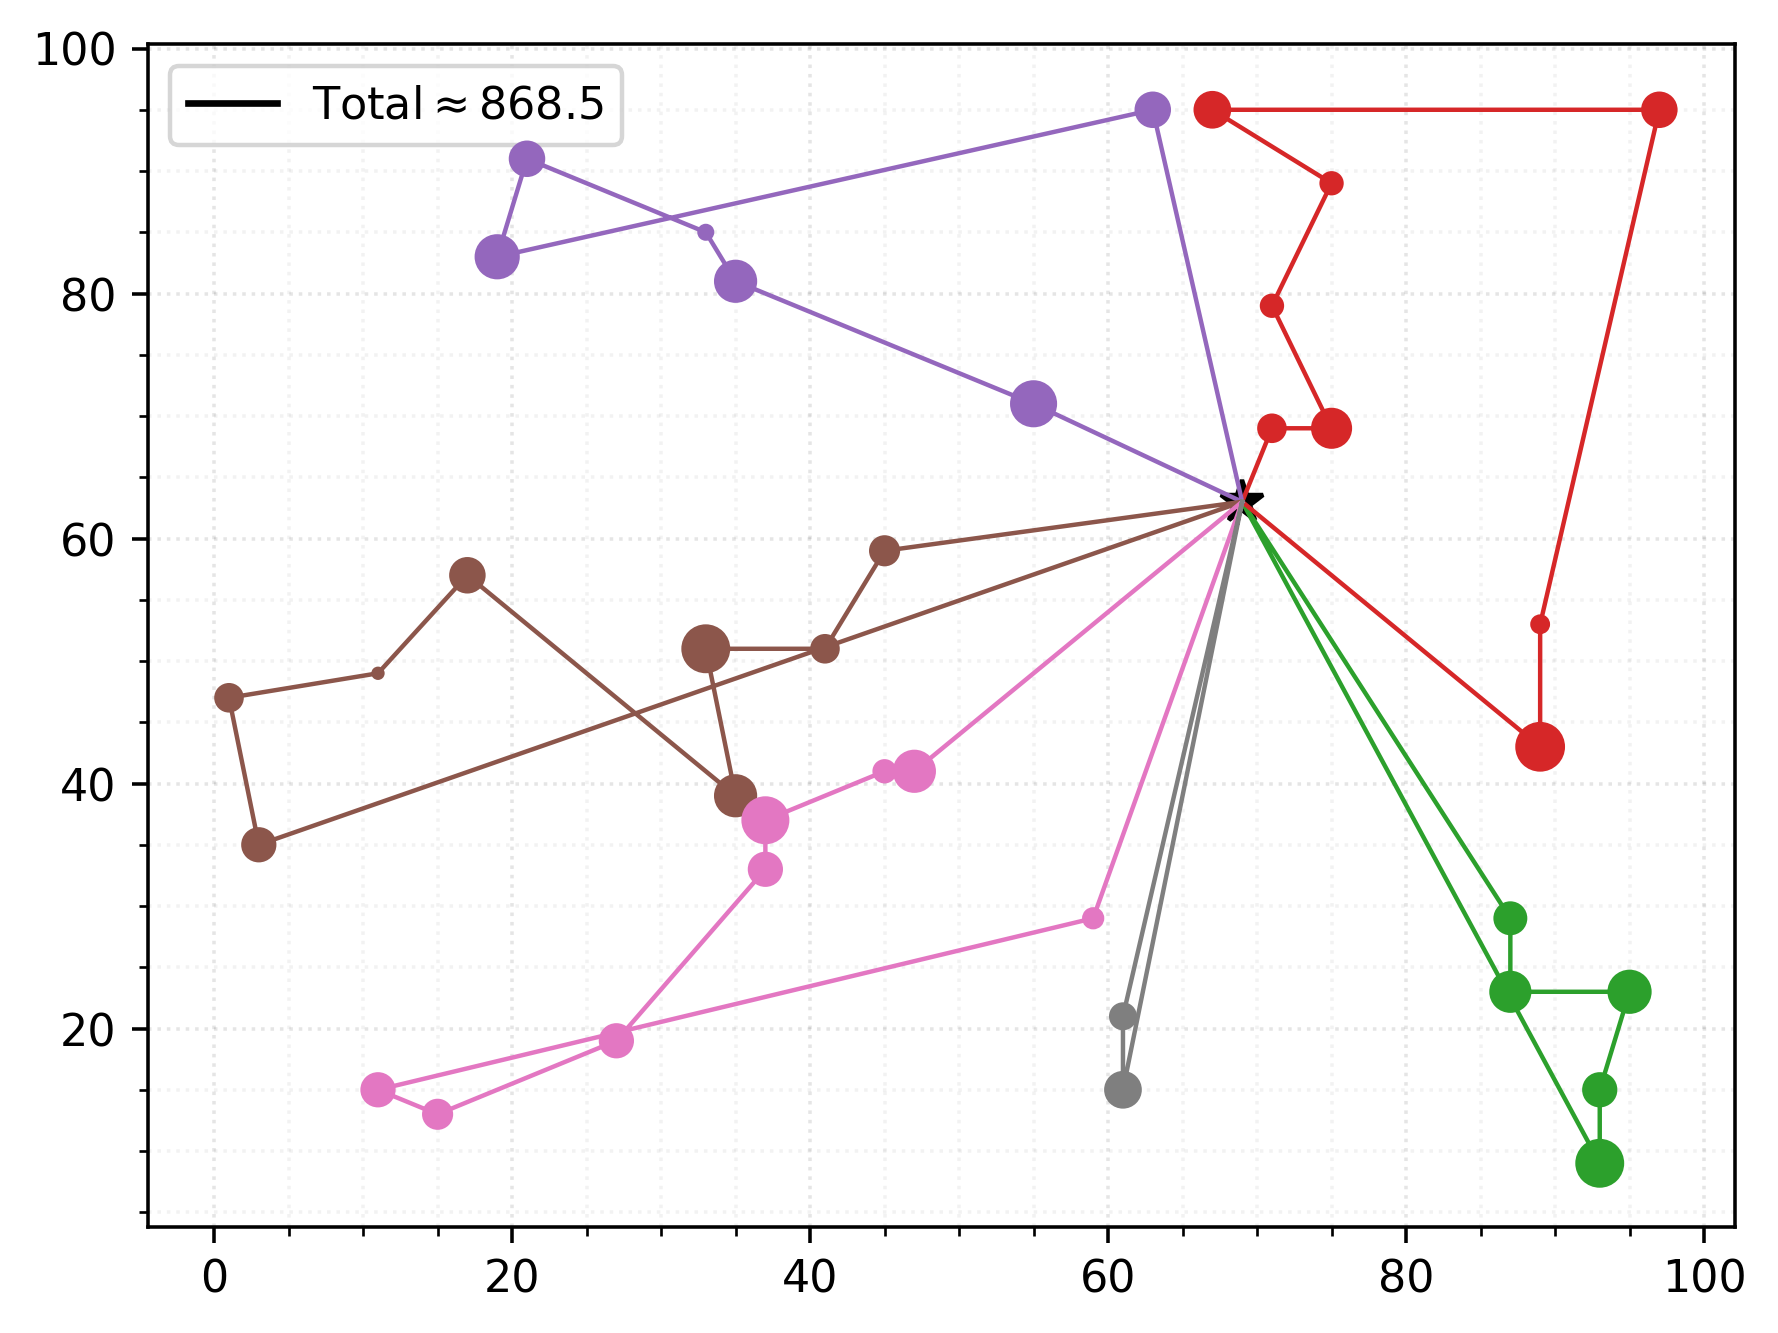
\includegraphics[width=\linewidth]{sweep/sw-A-n38-k5}\par
	\end{minipage}%
	\hspace{0.03\textwidth}
	\begin{minipage}{0.40\textwidth}
		\centering
		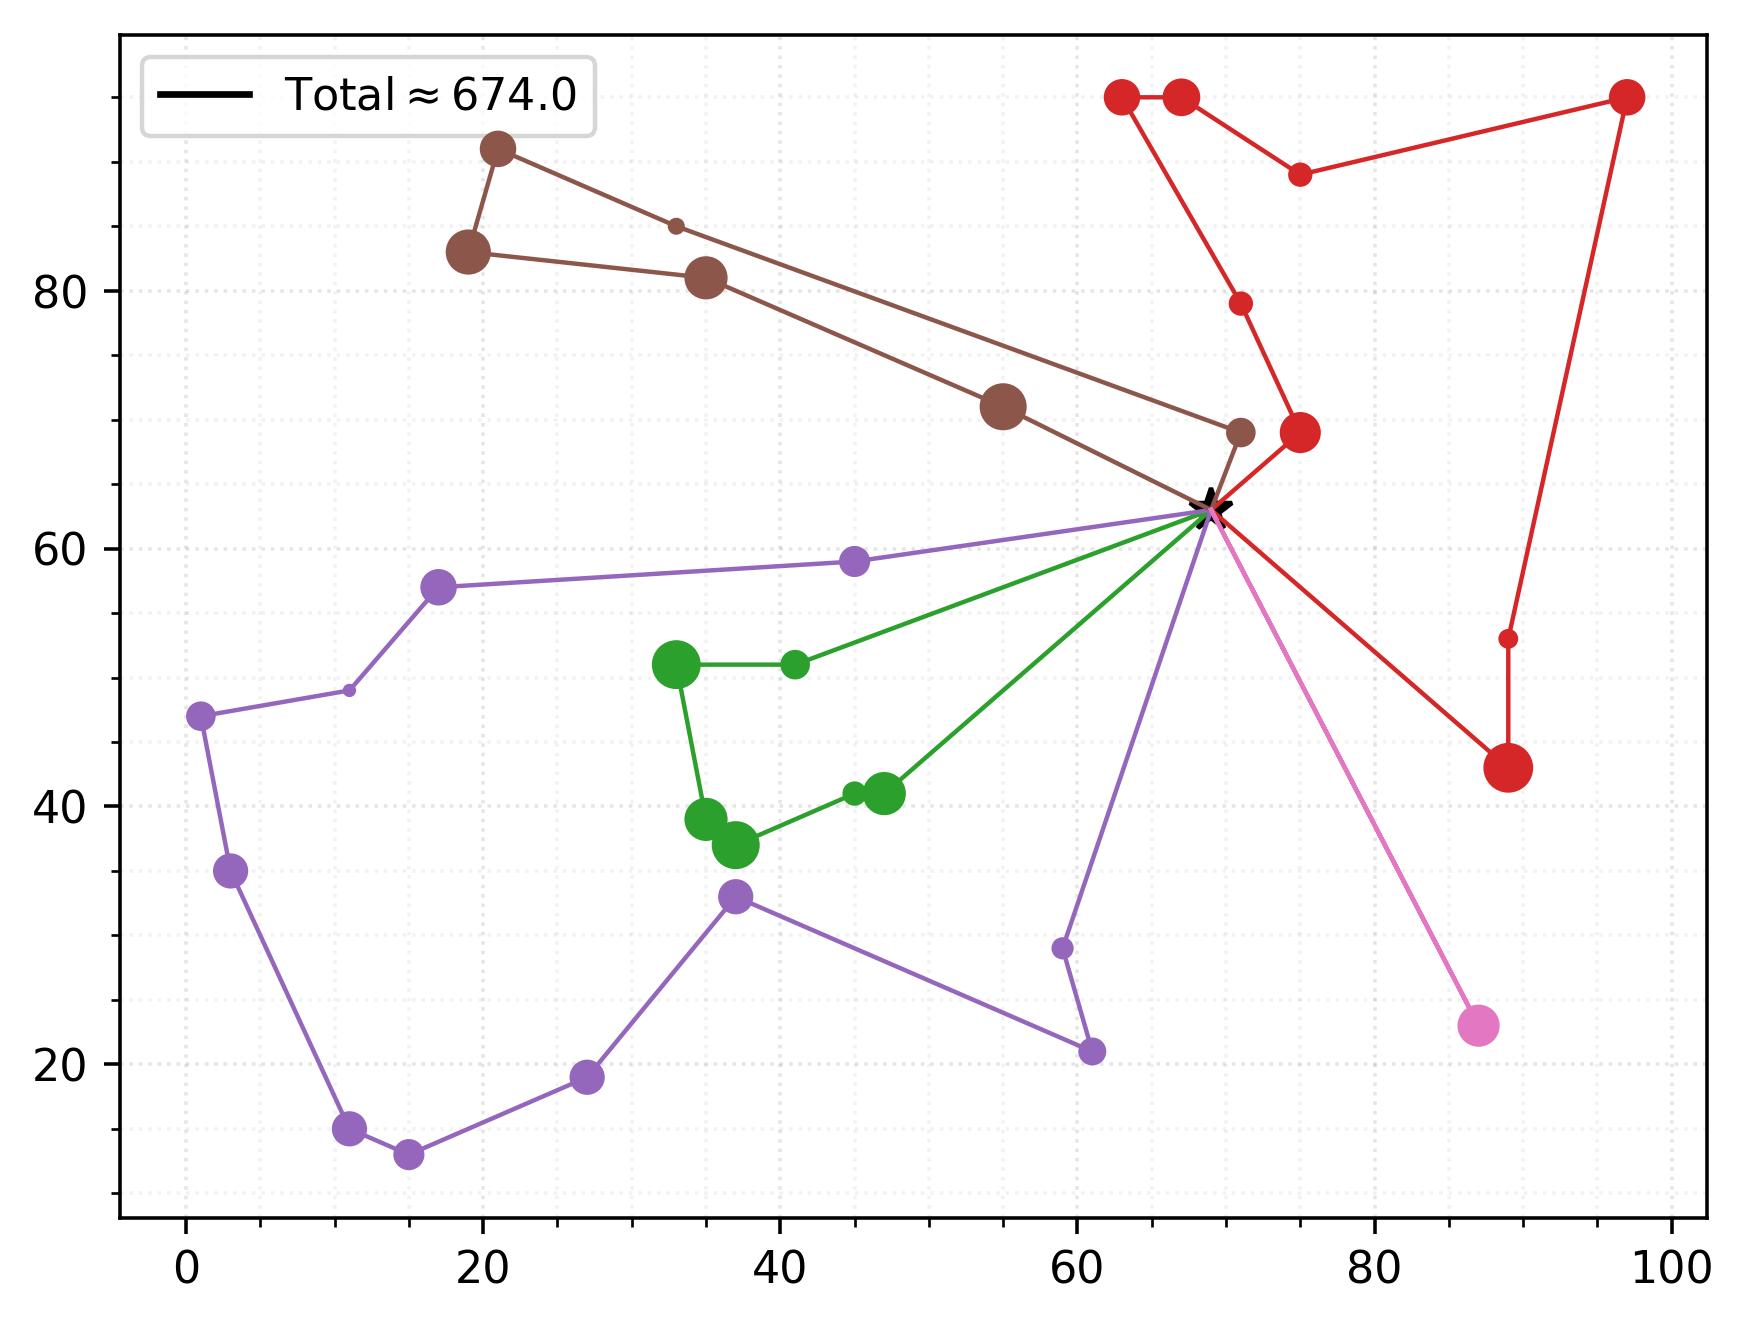
\includegraphics[width=\linewidth]{A-n38-k5-optima}\par
	\end{minipage}%
\end{figure}

\begin{figure}[H]
	\begin{minipage}{0.15\textwidth}
		\centering
		\texttt{A-n55-k9}
	\end{minipage}%
	\begin{minipage}{0.40\textwidth}
		\centering
		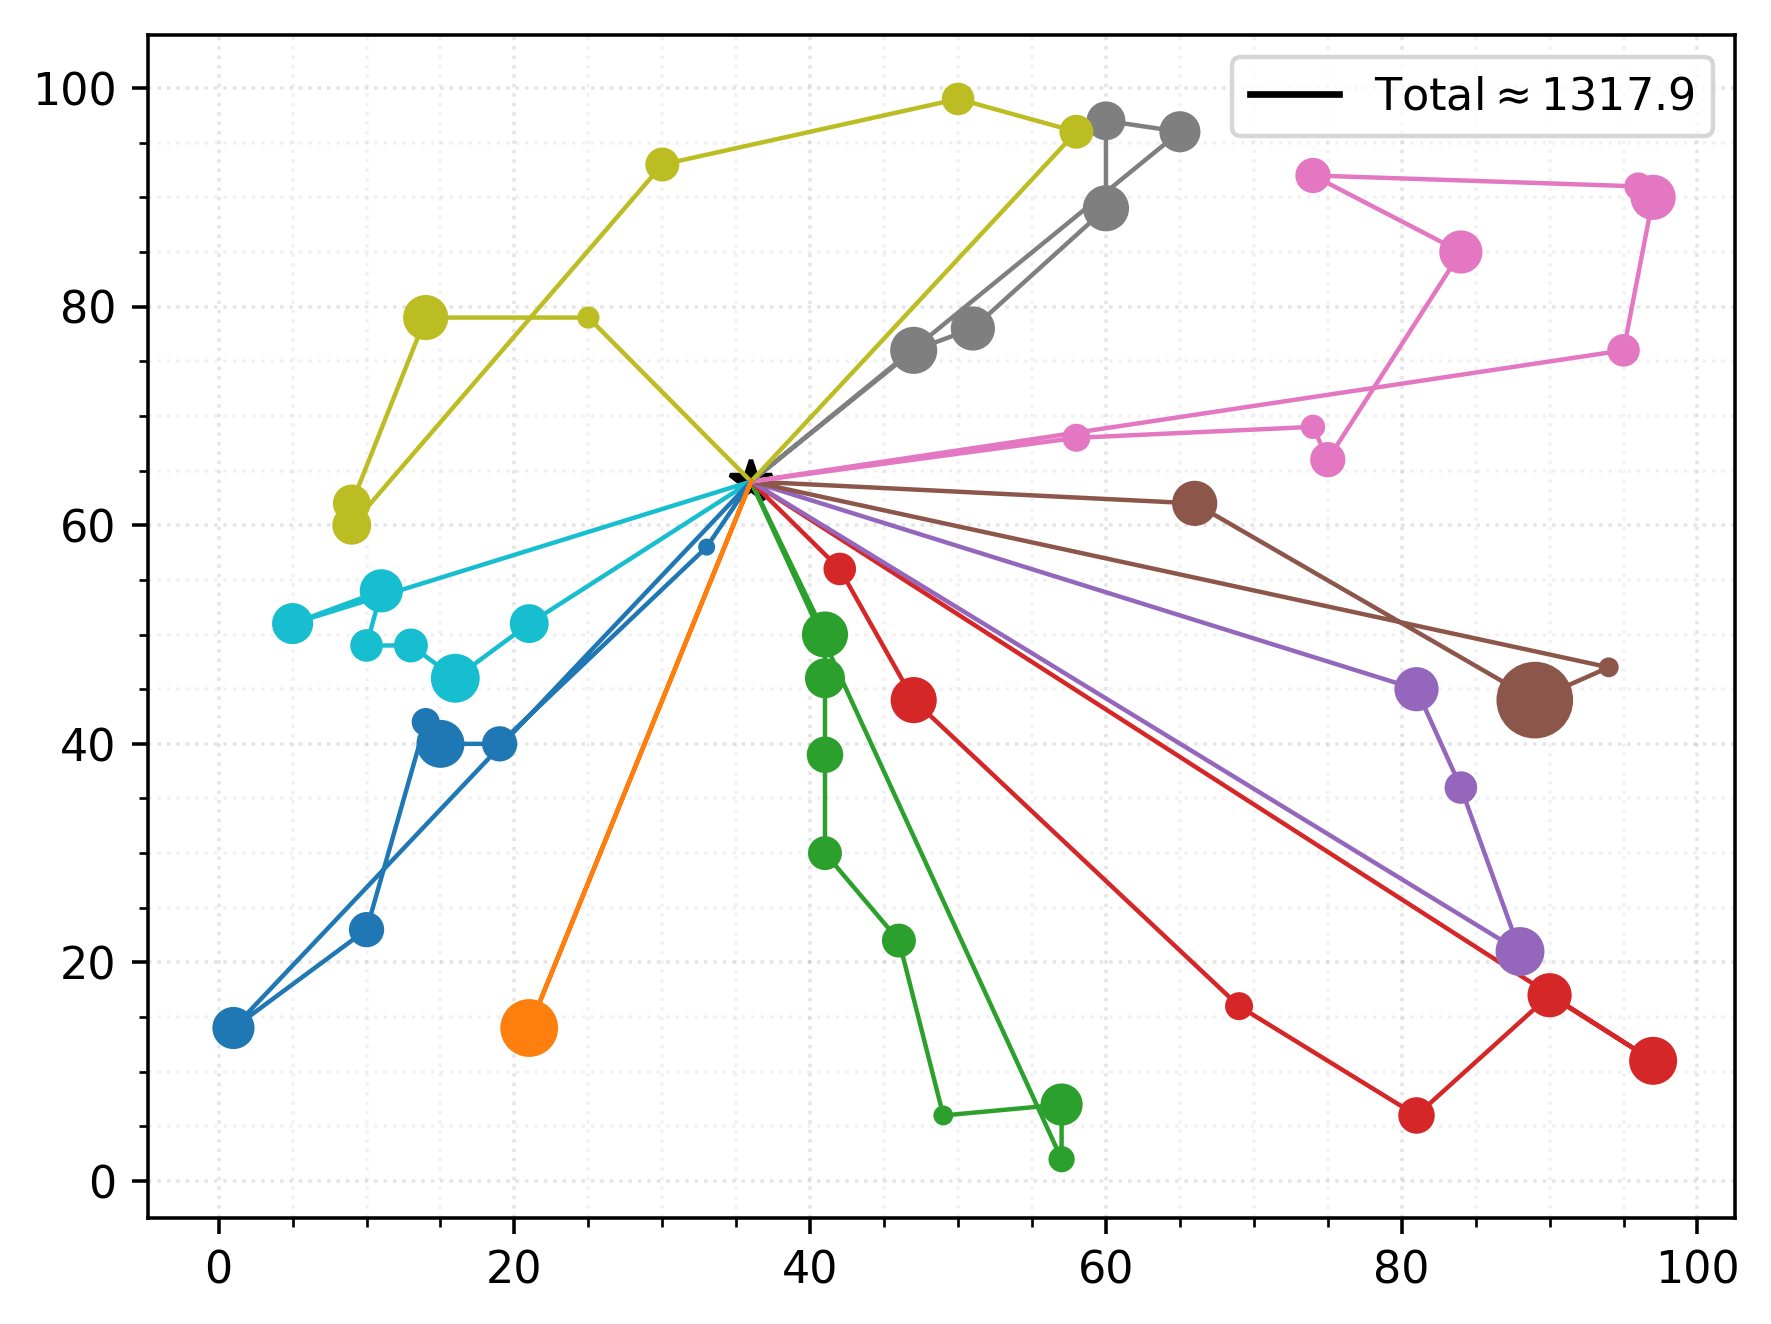
\includegraphics[width=\linewidth]{sweep/sw-A-n55-k9}\par
	\end{minipage}%
	\hspace{0.03\textwidth}
	\begin{minipage}{0.40\textwidth}
		\centering
		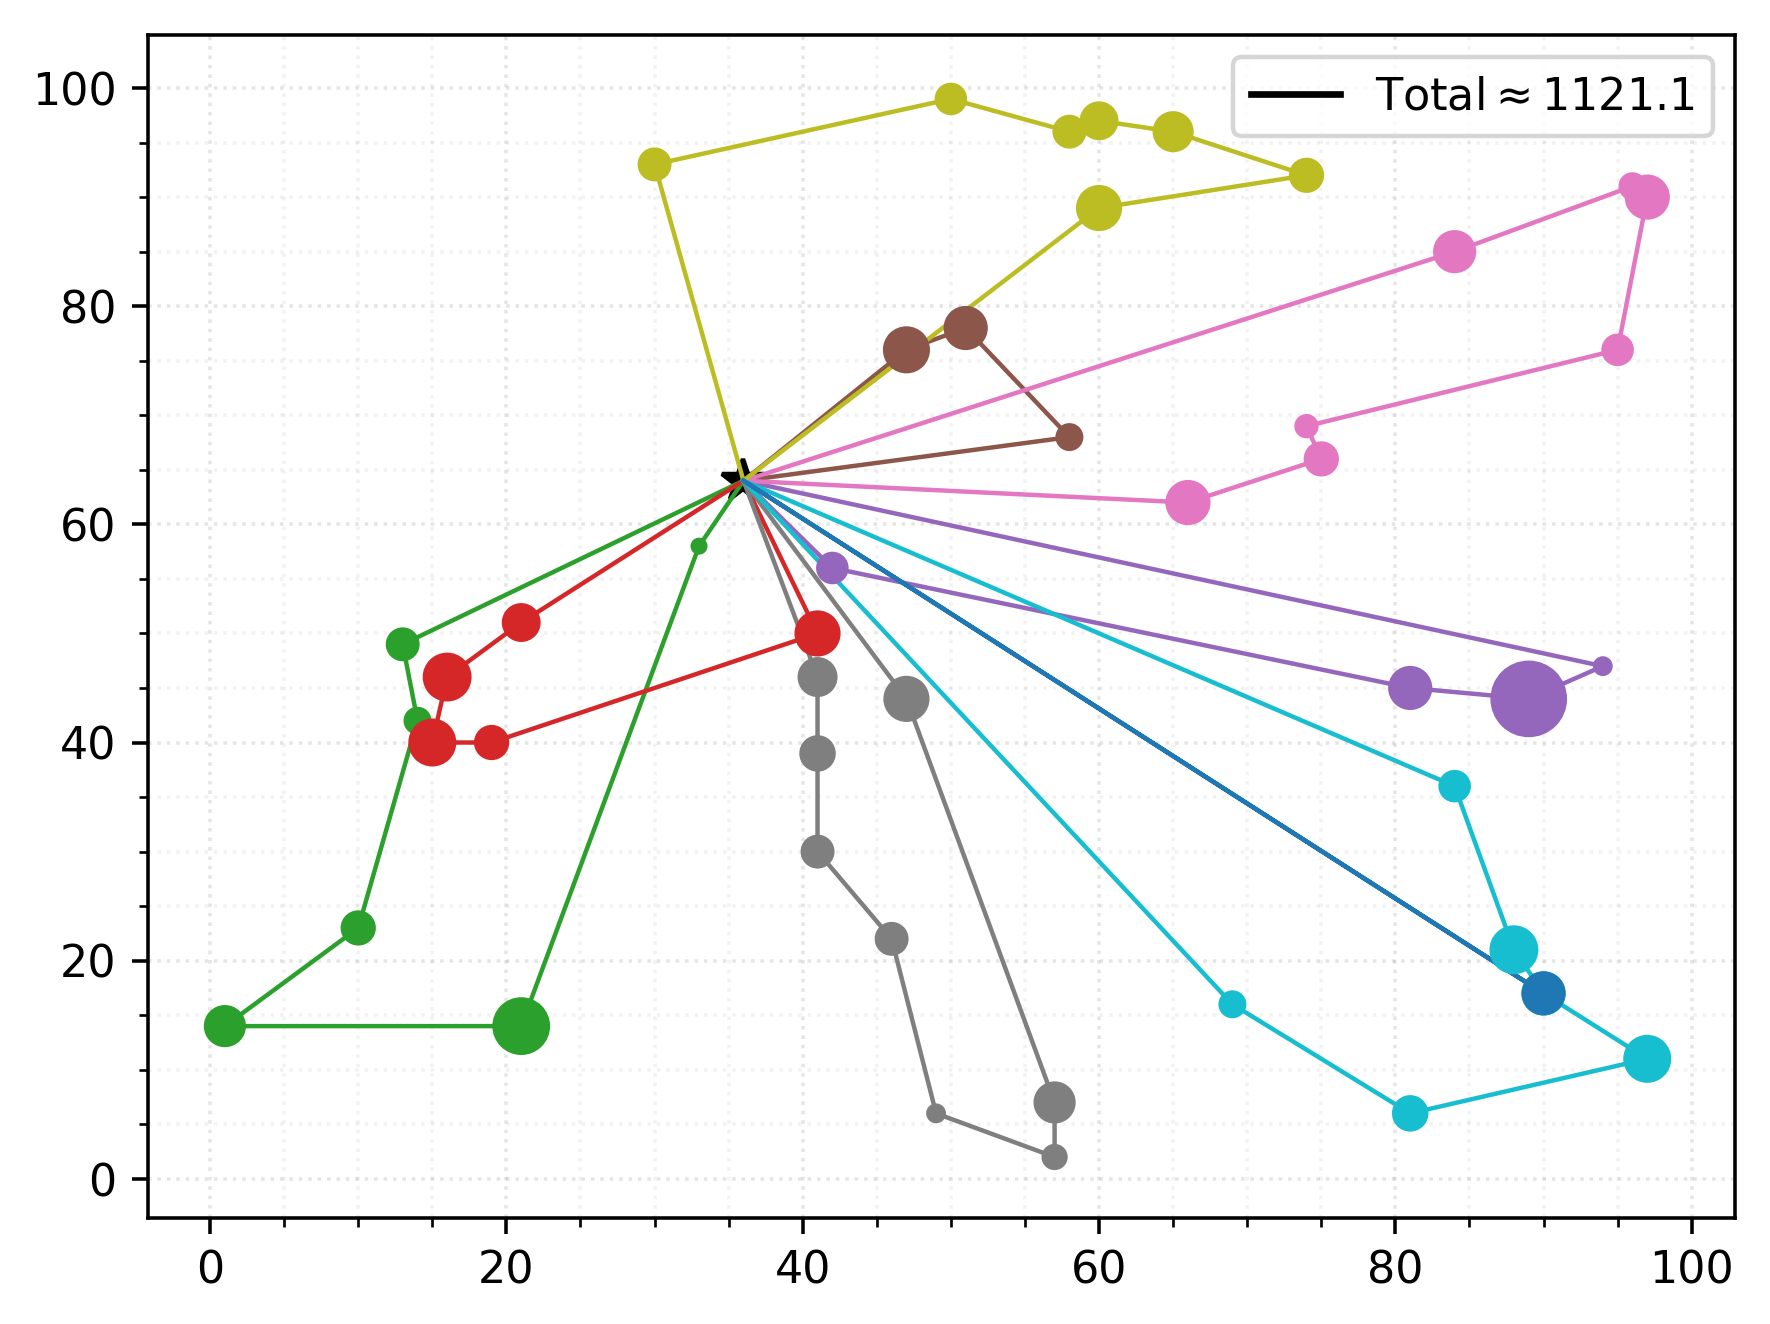
\includegraphics[width=\linewidth]{A-n55-k9-optima}\par
	\end{minipage}%
\end{figure}

\begin{figure}[H]
	\begin{minipage}{0.15\textwidth}
		\centering
		\texttt{B-n41-k6}
	\end{minipage}%
	\begin{minipage}{0.40\textwidth}
		\centering
		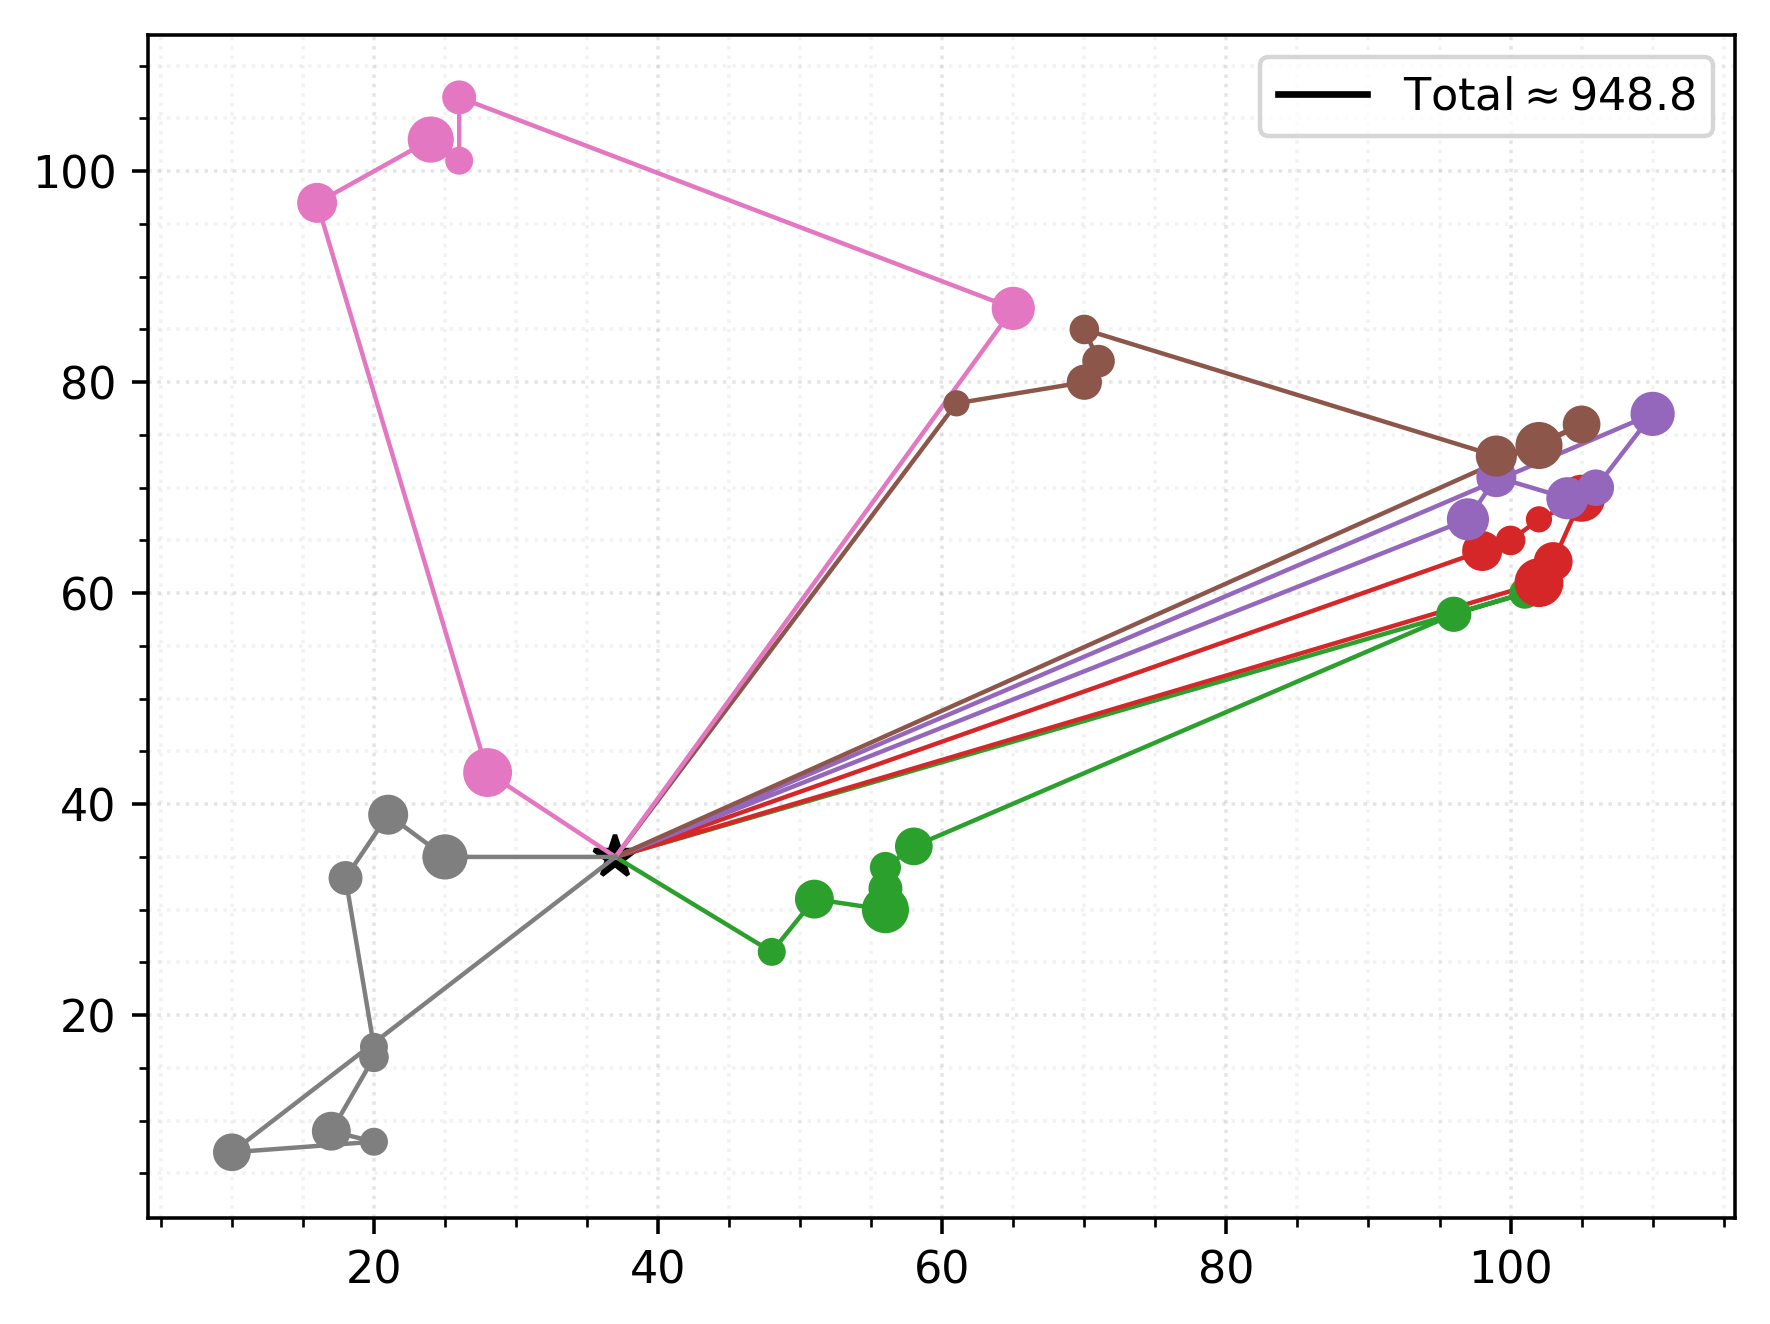
\includegraphics[width=\linewidth]{sweep/sw-B-n41-k6}\par
	\end{minipage}%
	\hspace{0.03\textwidth}
	\begin{minipage}{0.40\textwidth}
		\centering
		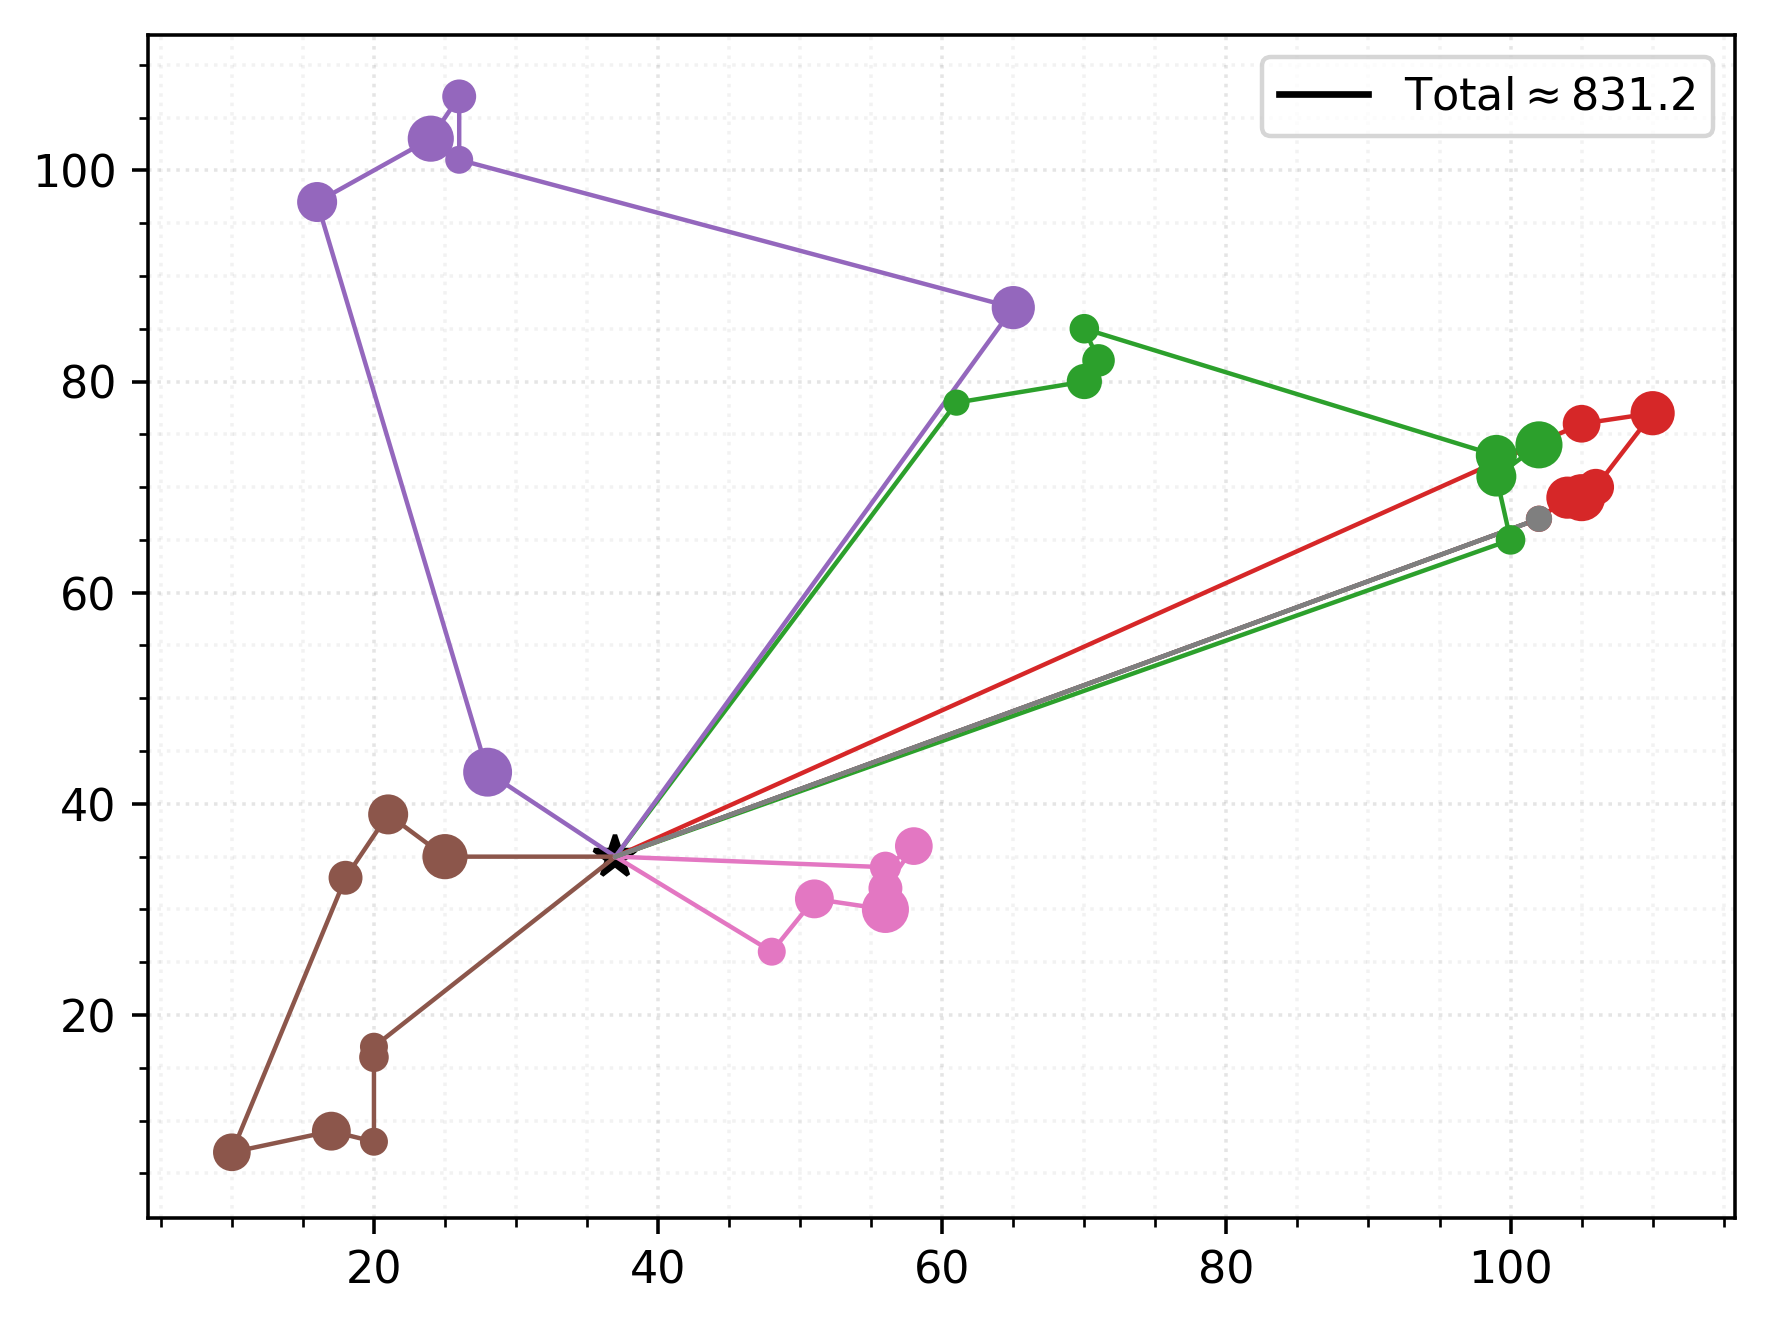
\includegraphics[width=\linewidth]{B-n41-k6-optima}\par
	\end{minipage}%
\end{figure}

\begin{figure}[H]
	\begin{minipage}{0.15\textwidth}
		\centering
		\texttt{B-n64-k9}
	\end{minipage}%
	\begin{minipage}{0.40\textwidth}
		\centering
		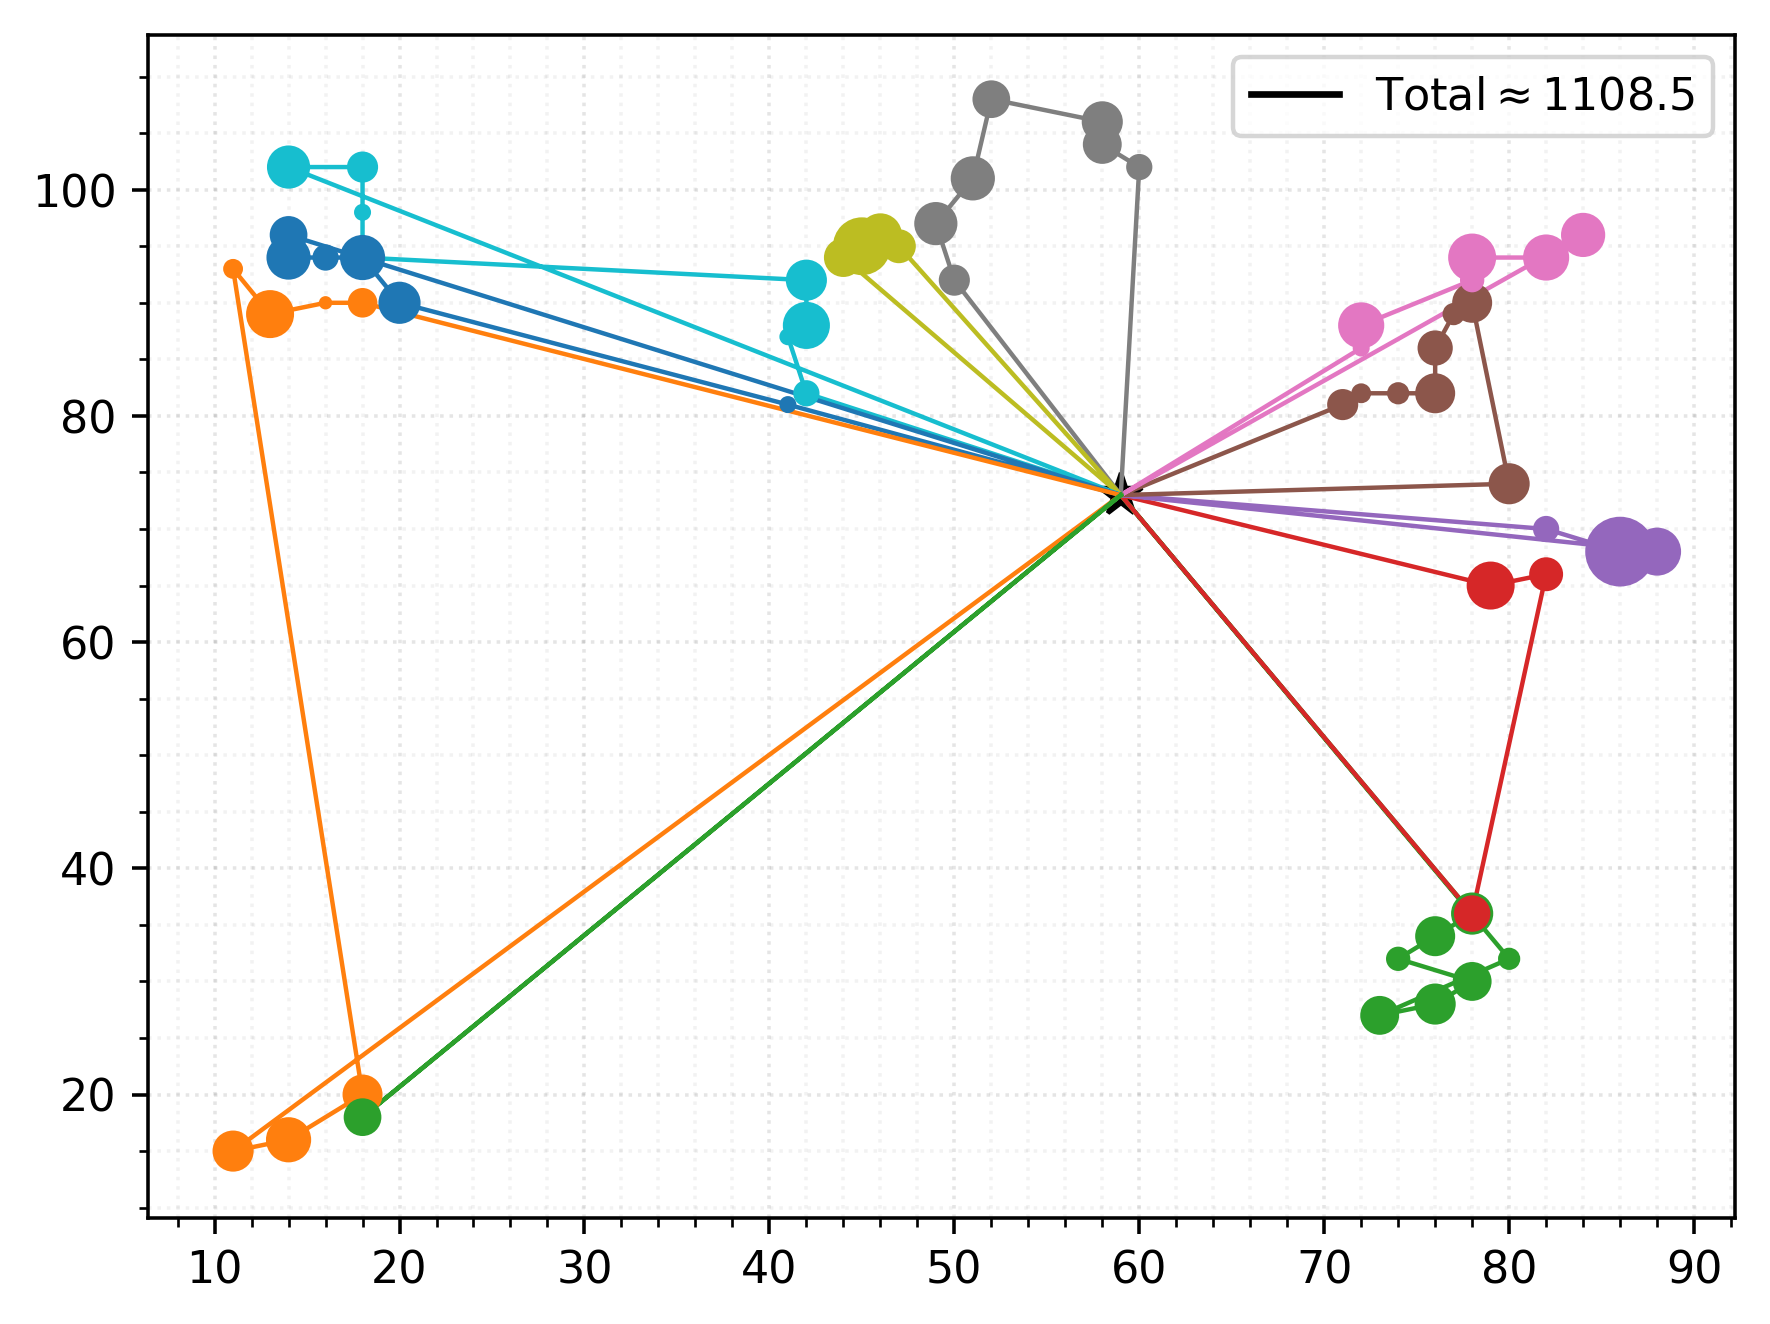
\includegraphics[width=\linewidth]{sweep/sw-B-n64-k9}\par
	\end{minipage}%
	\hspace{0.03\textwidth}
	\begin{minipage}{0.40\textwidth}
		\centering
		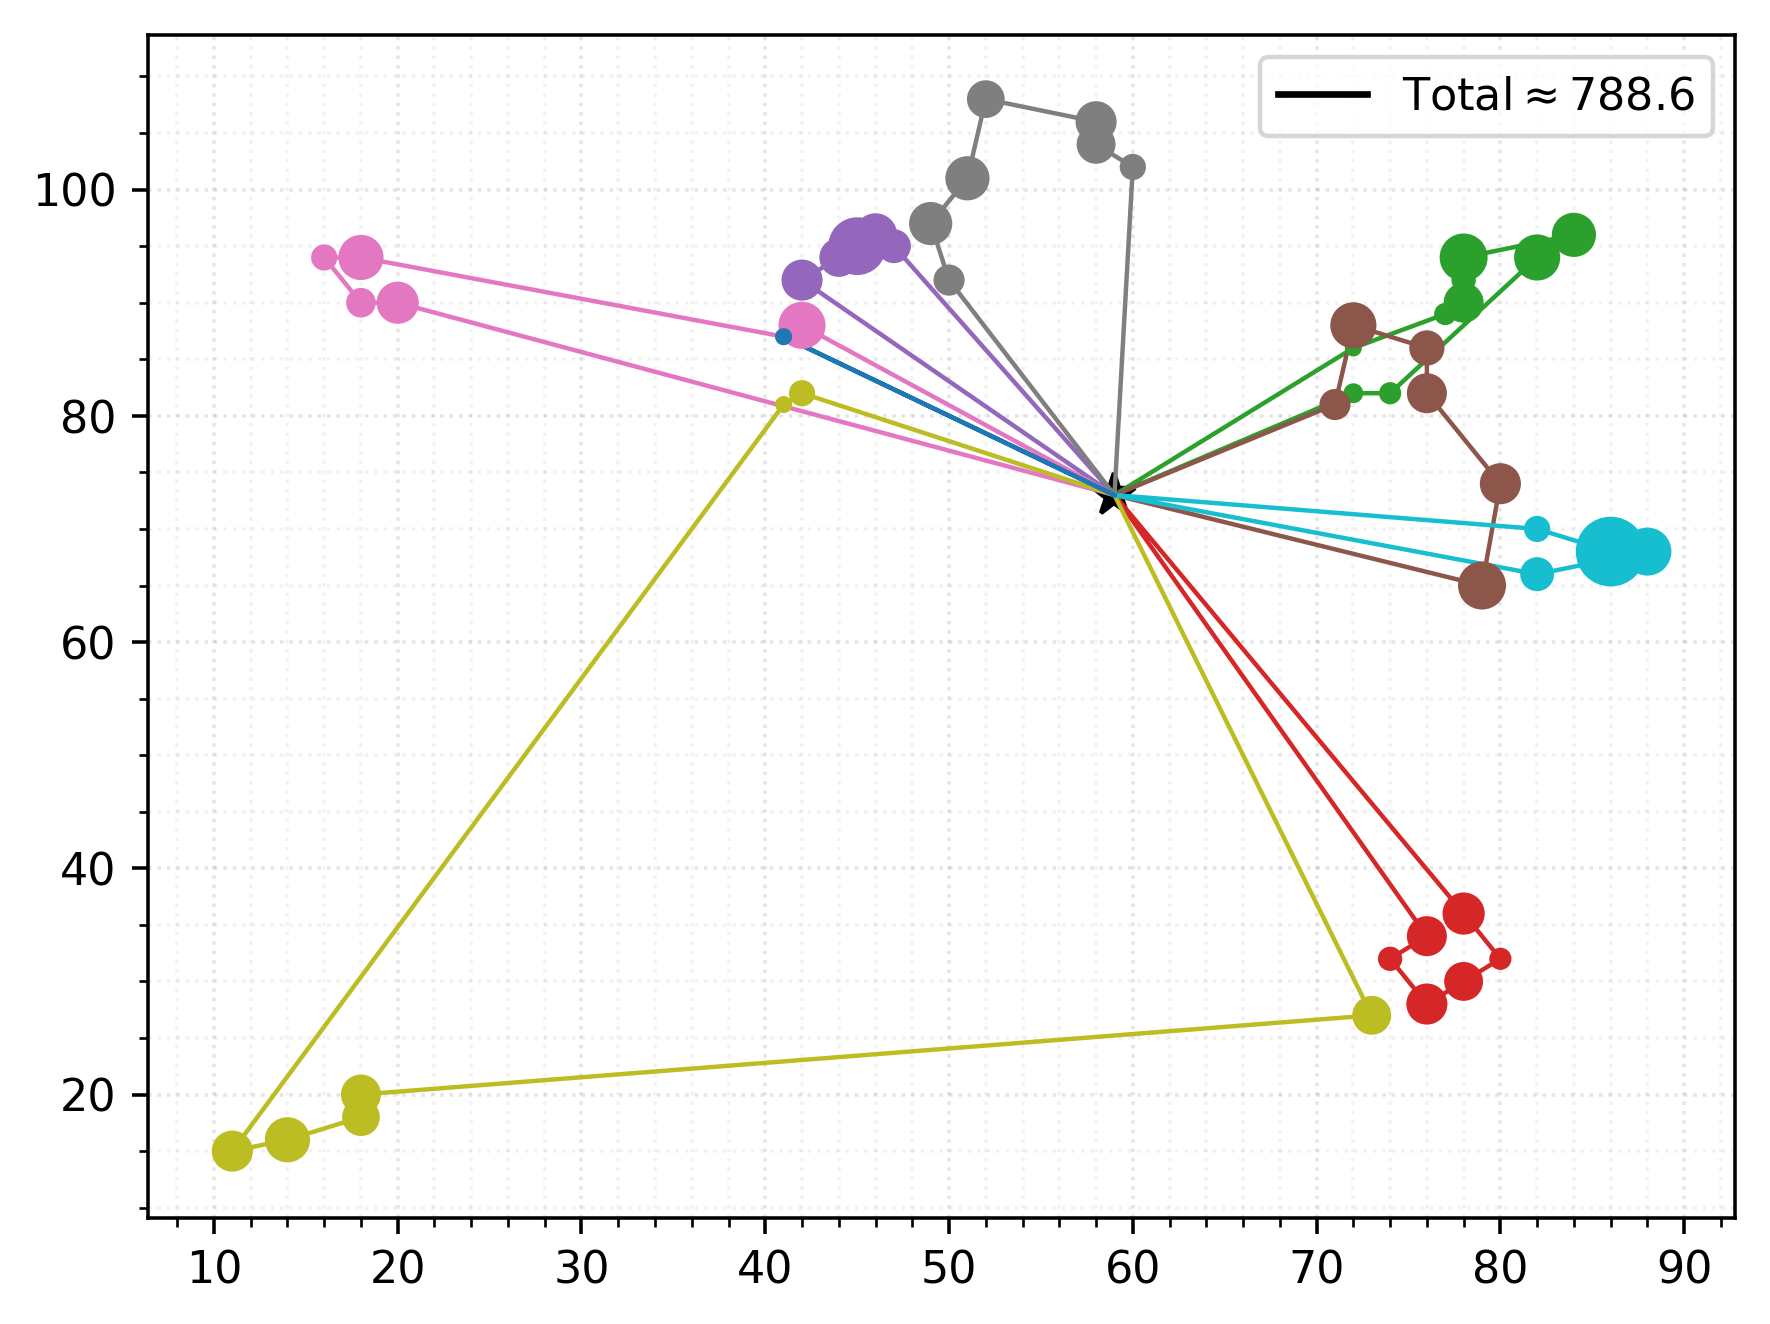
\includegraphics[width=\linewidth]{B-n64-k9-optima}\par
	\end{minipage}%
\end{figure}

\begin{figure}[H]
	\begin{minipage}{0.15\textwidth}
		\centering
		\texttt{B-n78-k10}
	\end{minipage}%
	\begin{minipage}{0.40\textwidth}
		\centering
		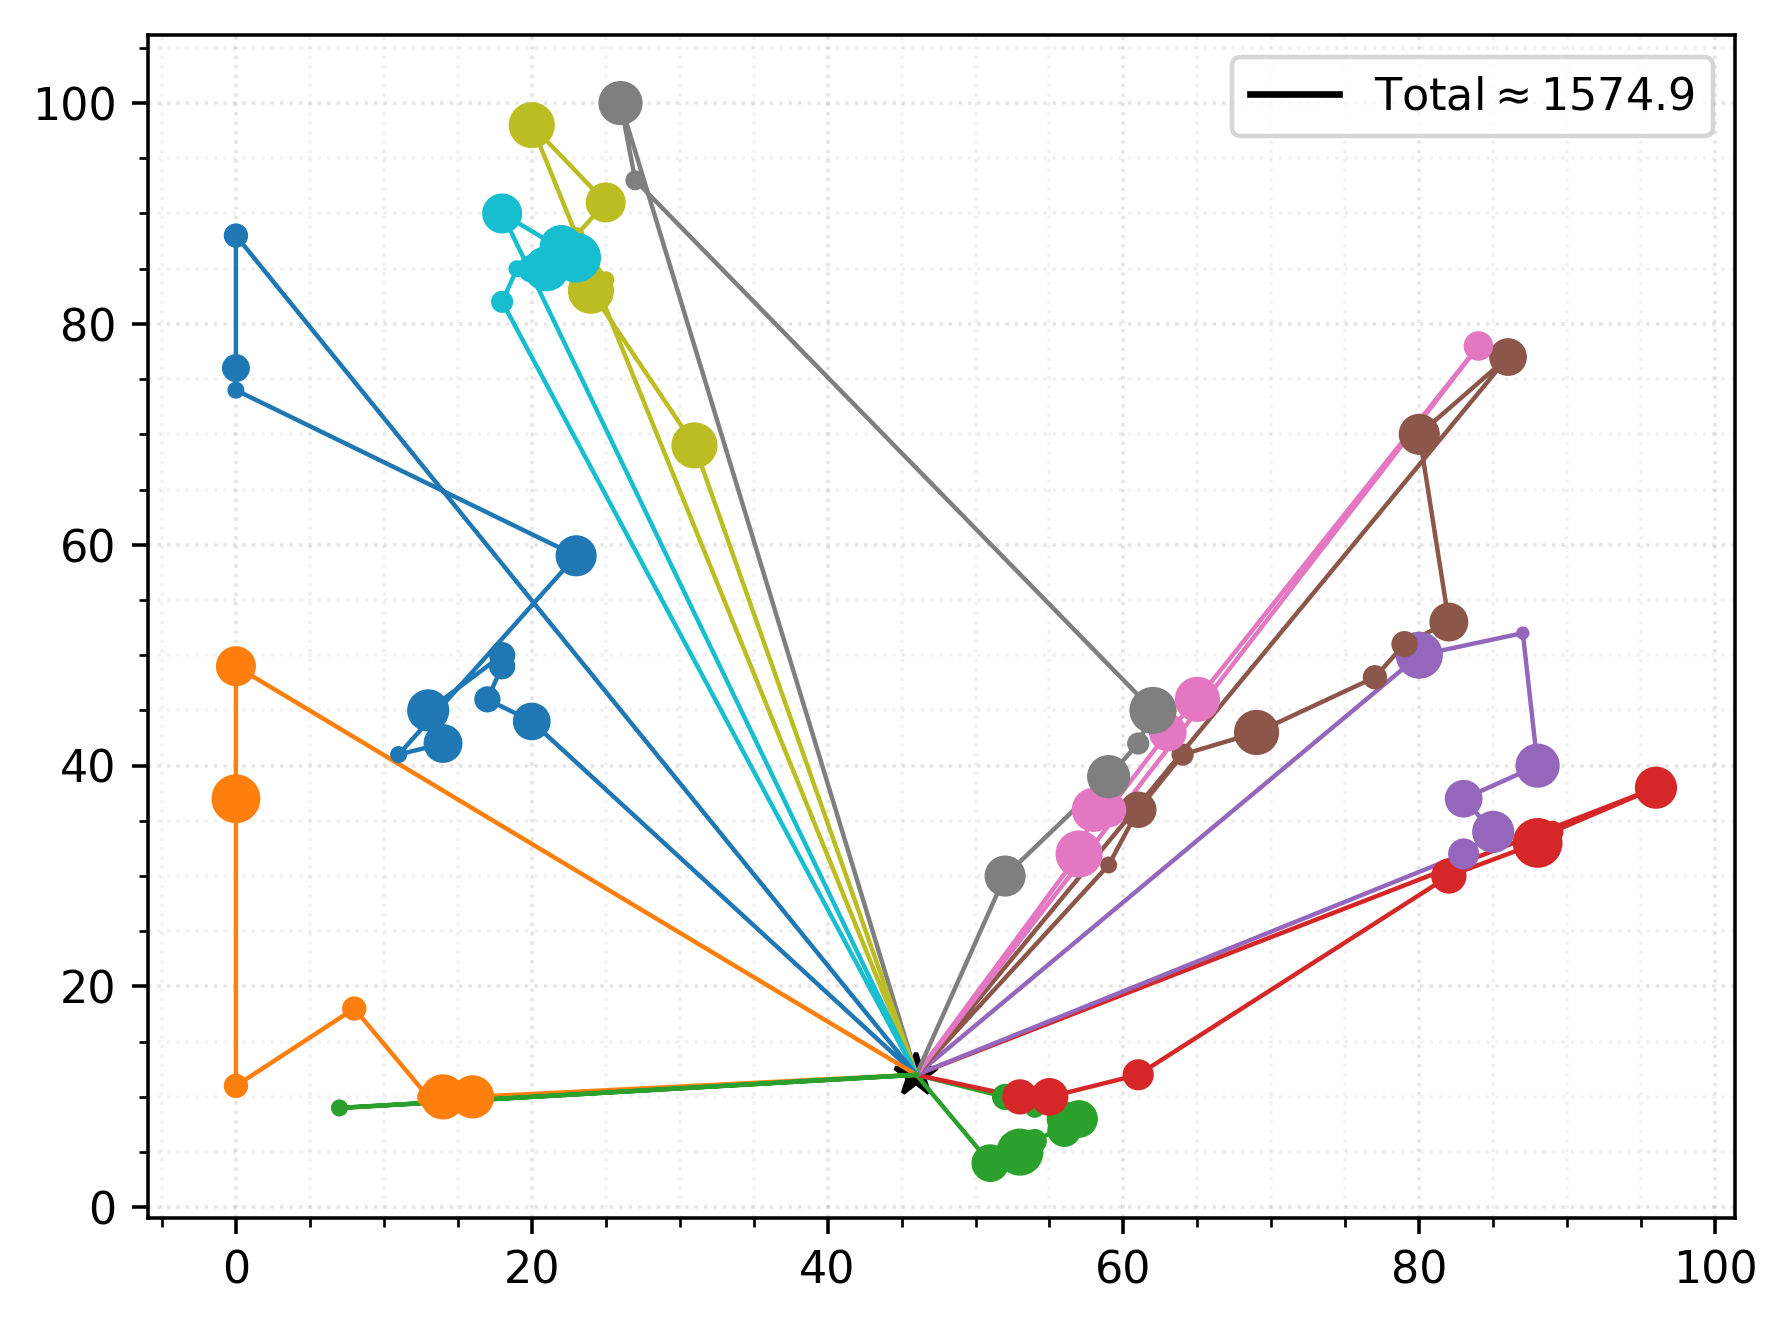
\includegraphics[width=\linewidth]{sweep/sw-B-n78-k10}\par
	\end{minipage}%
	\hspace{0.03\textwidth}
	\begin{minipage}{0.40\textwidth}
		\centering
		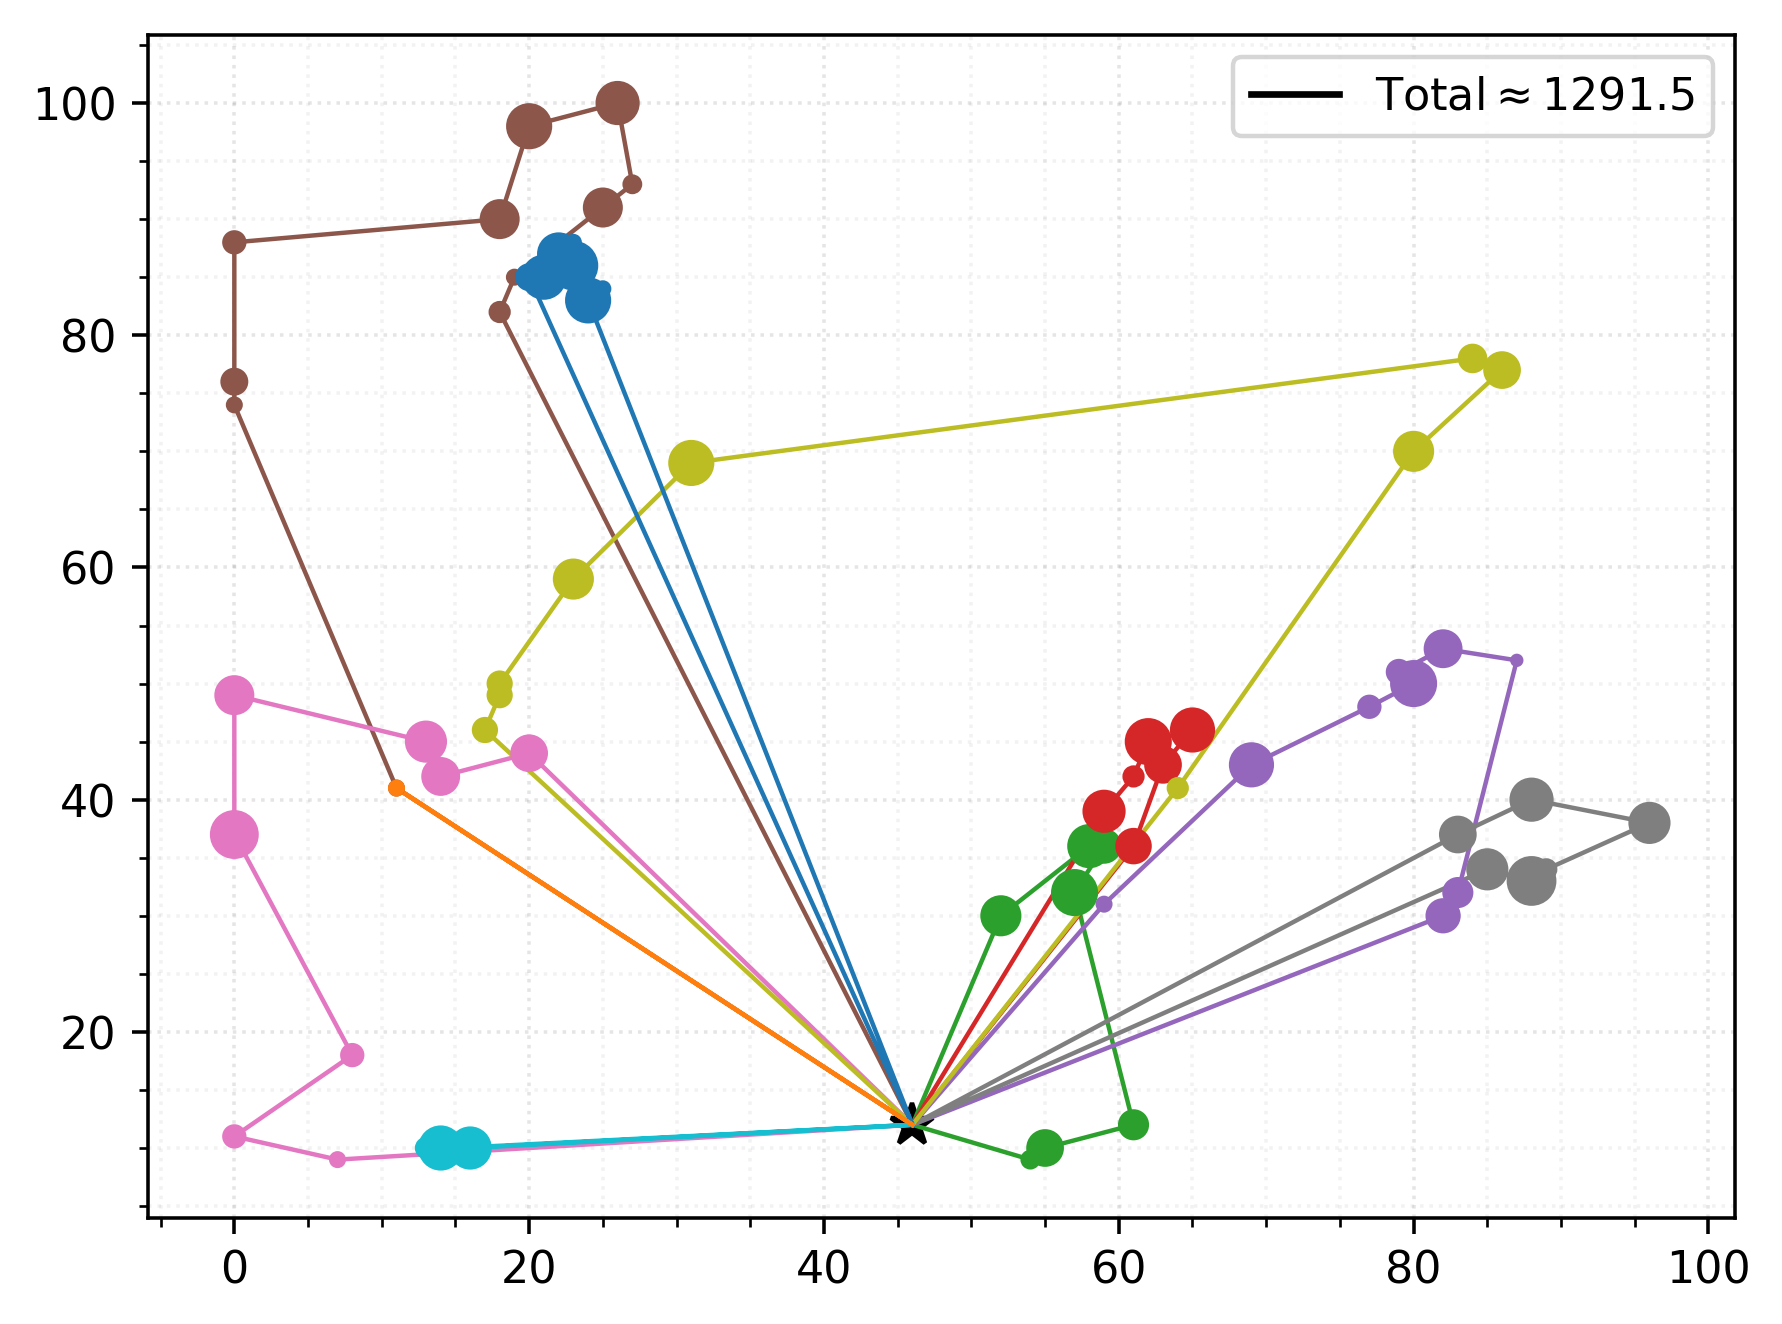
\includegraphics[width=\linewidth]{B-n78-k10-optima}\par
	\end{minipage}%
\end{figure}
